
%% bare_conf.tex
%% V1.3
%% 2007/01/11
%% by Michael Shell
%% See:
%% http://www.michaelshell.org/
%% for current contact information.
%%
%% This is a skeleton file demonstrating the use of IEEEtran.cls
%% (requires IEEEtran.cls version 1.7 or later) with an IEEE conference paper.
%%
%% Support sites:
%% http://www.michaelshell.org/tex/ieeetran/
%% http://www.ctan.org/tex-archive/macros/latex/contrib/IEEEtran/
%% and
%% http://www.ieee.org/

%%*************************************************************************
%% Legal Notice:
%% This code is offered as-is without any warranty either expressed or
%% implied; without even the implied warranty of MERCHANTABILITY or
%% FITNESS FOR A PARTICULAR PURPOSE! 
%% User assumes all risk.
%% In no event shall IEEE or any contributor to this code be liable for
%% any damages or losses, including, but not limited to, incidental,
%% consequential, or any other damages, resulting from the use or misuse
%% of any information contained here.
%%
%% All comments are the opinions of their respective authors and are not
%% necessarily endorsed by the IEEE.
%%
%% This work is distributed under the LaTeX Project Public License (LPPL)
%% ( http://www.latex-project.org/ ) version 1.3, and may be freely used,
%% distributed and modified. A copy of the LPPL, version 1.3, is included
%% in the base LaTeX documentation of all distributions of LaTeX released
%% 2003/12/01 or later.
%% Retain all contribution notices and credits.
%% ** Modified files should be clearly indicated as such, including  **
%% ** renaming them and changing author support contact information. **
%%
%% File list of work: IEEEtran.cls, IEEEtran_HOWTO.pdf, bare_adv.tex,
%%                    bare_conf.tex, bare_jrnl.tex, bare_jrnl_compsoc.tex
%%*************************************************************************

% *** Authors should verify (and, if needed, correct) their LaTeX system  ***
% *** with the testflow diagnostic prior to trusting their LaTeX platform ***
% *** with production work. IEEE's font choices can trigger bugs that do  ***
% *** not appear when using other class files.                            ***
% The testflow support page is at:
% http://www.michaelshell.org/tex/testflow/



% Note that the a4paper option is mainly intended so that authors in
% countries using A4 can easily print to A4 and see how their papers will
% look in print - the typesetting of the document will not typically be
% affected with changes in paper size (but the bottom and side margins will).
% Use the testflow package mentioned above to verify correct handling of
% both paper sizes by the user's LaTeX system.
%
% Also note that the "draftcls" or "draftclsnofoot", not "draft", option
% should be used if it is desired that the figures are to be displayed in
% draft mode.
%
\documentclass[conference]{IEEEtran}
% Add the compsoc option for Computer Society conferences.
%
% If IEEEtran.cls has not been installed into the LaTeX system files,
% manually specify the path to it like:
% \documentclass[conference]{../sty/IEEEtran}





% Some very useful LaTeX packages include:
% (uncomment the ones you want to load)


% *** MISC UTILITY PACKAGES ***
%
%\usepackage{ifpdf}
% Heiko Oberdiek's ifpdf.sty is very useful if you need conditional
% compilation based on whether the output is pdf or dvi.
% usage:
% \ifpdf
%   % pdf code
% \else
%   % dvi code
% \fi
% The latest version of ifpdf.sty can be obtained from:
% http://www.ctan.org/tex-archive/macros/latex/contrib/oberdiek/
% Also, note that IEEEtran.cls V1.7 and later provides a builtin
% \ifCLASSINFOpdf conditional that works the same way.
% When switching from latex to pdflatex and vice-versa, the compiler may
% have to be run twice to clear warning/error messages.






% *** CITATION PACKAGES ***
%
%\usepackage{cite}
% cite.sty was written by Donald Arseneau
% V1.6 and later of IEEEtran pre-defines the format of the cite.sty package
% \cite{} output to follow that of IEEE. Loading the cite package will
% result in citation numbers being automatically sorted and properly
% "compressed/ranged". e.g., [1], [9], [2], [7], [5], [6] without using
% cite.sty will become [1], [2], [5]--[7], [9] using cite.sty. cite.sty's
% \cite will automatically add leading space, if needed. Use cite.sty's
% noadjust option (cite.sty V3.8 and later) if you want to turn this off.
% cite.sty is already installed on most LaTeX systems. Be sure and use
% version 4.0 (2003-05-27) and later if using hyperref.sty. cite.sty does
% not currently provide for hyperlinked citations.
% The latest version can be obtained at:
% http://www.ctan.org/tex-archive/macros/latex/contrib/cite/
% The documentation is contained in the cite.sty file itself.






% *** GRAPHICS RELATED PACKAGES ***
%
\ifCLASSINFOpdf
  % \usepackage[pdftex]{graphicx}
  % declare the path(s) where your graphic files are
  % \graphicspath{{../pdf/}{../jpeg/}}
  % and their extensions so you won't have to specify these with
  % every instance of \includegraphics
  % \DeclareGraphicsExtensions{.pdf,.jpeg,.png}
\else
  % or other class option (dvipsone, dvipdf, if not using dvips). graphicx
  % will default to the driver specified in the system graphics.cfg if no
  % driver is specified.
  % \usepackage[dvips]{graphicx}
  % declare the path(s) where your graphic files are
  % \graphicspath{{../eps/}}
  % and their extensions so you won't have to specify these with
  % every instance of \includegraphics
  % \DeclareGraphicsExtensions{.eps}
\fi
% graphicx was written by David Carlisle and Sebastian Rahtz. It is
% required if you want graphics, photos, etc. graphicx.sty is already
% installed on most LaTeX systems. The latest version and documentation can
% be obtained at: 
% http://www.ctan.org/tex-archive/macros/latex/required/graphics/
% Another good source of documentation is "Using Imported Graphics in
% LaTeX2e" by Keith Reckdahl which can be found as epslatex.ps or
% epslatex.pdf at: http://www.ctan.org/tex-archive/info/
%
% latex, and pdflatex in dvi mode, support graphics in encapsulated
% postscript (.eps) format. pdflatex in pdf mode supports graphics
% in .pdf, .jpeg, .png and .mps (metapost) formats. Users should ensure
% that all non-photo figures use a vector format (.eps, .pdf, .mps) and
% not a bitmapped formats (.jpeg, .png). IEEE frowns on bitmapped formats
% which can result in "jaggedy"/blurry rendering of lines and letters as
% well as large increases in file sizes.
%
% You can find documentation about the pdfTeX application at:
% http://www.tug.org/applications/pdftex





% *** MATH PACKAGES ***
%
%\usepackage[cmex10]{amsmath}
% A popular package from the American Mathematical Society that provides
% many useful and powerful commands for dealing with mathematics. If using
% it, be sure to load this package with the cmex10 option to ensure that
% only type 1 fonts will utilized at all point sizes. Without this option,
% it is possible that some math symbols, particularly those within
% footnotes, will be rendered in bitmap form which will result in a
% document that can not be IEEE Xplore compliant!
%
% Also, note that the amsmath package sets \interdisplaylinepenalty to 10000
% thus preventing page breaks from occurring within multiline equations. Use:
%\interdisplaylinepenalty=2500
% after loading amsmath to restore such page breaks as IEEEtran.cls normally
% does. amsmath.sty is already installed on most LaTeX systems. The latest
% version and documentation can be obtained at:
% http://www.ctan.org/tex-archive/macros/latex/required/amslatex/math/





% *** SPECIALIZED LIST PACKAGES ***
%
%\usepackage{algorithmic}
% algorithmic.sty was written by Peter Williams and Rogerio Brito.
% This package provides an algorithmic environment fo describing algorithms.
% You can use the algorithmic environment in-text or within a figure
% environment to provide for a floating algorithm. Do NOT use the algorithm
% floating environment provided by algorithm.sty (by the same authors) or
% algorithm2e.sty (by Christophe Fiorio) as IEEE does not use dedicated
% algorithm float types and packages that provide these will not provide
% correct IEEE style captions. The latest version and documentation of
% algorithmic.sty can be obtained at:
% http://www.ctan.org/tex-archive/macros/latex/contrib/algorithms/
% There is also a support site at:
% http://algorithms.berlios.de/index.html
% Also of interest may be the (relatively newer and more customizable)
% algorithmicx.sty package by Szasz Janos:
% http://www.ctan.org/tex-archive/macros/latex/contrib/algorithmicx/




% *** ALIGNMENT PACKAGES ***
%
%\usepackage{array}
% Frank Mittelbach's and David Carlisle's array.sty patches and improves
% the standard LaTeX2e array and tabular environments to provide better
% appearance and additional user controls. As the default LaTeX2e table
% generation code is lacking to the point of almost being broken with
% respect to the quality of the end results, all users are strongly
% advised to use an enhanced (at the very least that provided by array.sty)
% set of table tools. array.sty is already installed on most systems. The
% latest version and documentation can be obtained at:
% http://www.ctan.org/tex-archive/macros/latex/required/tools/


%\usepackage{mdwmath}
%\usepackage{mdwtab}
% Also highly recommended is Mark Wooding's extremely powerful MDW tools,
% especially mdwmath.sty and mdwtab.sty which are used to format equations
% and tables, respectively. The MDWtools set is already installed on most
% LaTeX systems. The lastest version and documentation is available at:
% http://www.ctan.org/tex-archive/macros/latex/contrib/mdwtools/


% IEEEtran contains the IEEEeqnarray family of commands that can be used to
% generate multiline equations as well as matrices, tables, etc., of high
% quality.


%\usepackage{eqparbox}
% Also of notable interest is Scott Pakin's eqparbox package for creating
% (automatically sized) equal width boxes - aka "natural width parboxes".
% Available at:
% http://www.ctan.org/tex-archive/macros/latex/contrib/eqparbox/





% *** SUBFIGURE PACKAGES ***
%\usepackage[tight,footnotesize]{subfigure}
% subfigure.sty was written by Steven Douglas Cochran. This package makes it
% easy to put subfigures in your figures. e.g., "Figure 1a and 1b". For IEEE
% work, it is a good idea to load it with the tight package option to reduce
% the amount of white space around the subfigures. subfigure.sty is already
% installed on most LaTeX systems. The latest version and documentation can
% be obtained at:
% http://www.ctan.org/tex-archive/obsolete/macros/latex/contrib/subfigure/
% subfigure.sty has been superceeded by subfig.sty.



%\usepackage[caption=false]{caption}
%\usepackage[font=footnotesize]{subfig}
% subfig.sty, also written by Steven Douglas Cochran, is the modern
% replacement for subfigure.sty. However, subfig.sty requires and
% automatically loads Axel Sommerfeldt's caption.sty which will override
% IEEEtran.cls handling of captions and this will result in nonIEEE style
% figure/table captions. To prevent this problem, be sure and preload
% caption.sty with its "caption=false" package option. This is will preserve
% IEEEtran.cls handing of captions. Version 1.3 (2005/06/28) and later 
% (recommended due to many improvements over 1.2) of subfig.sty supports
% the caption=false option directly:
%\usepackage[caption=false,font=footnotesize]{subfig}
%
% The latest version and documentation can be obtained at:
% http://www.ctan.org/tex-archive/macros/latex/contrib/subfig/
% The latest version and documentation of caption.sty can be obtained at:
% http://www.ctan.org/tex-archive/macros/latex/contrib/caption/




% *** FLOAT PACKAGES ***
%
%\usepackage{fixltx2e}
% fixltx2e, the successor to the earlier fix2col.sty, was written by
% Frank Mittelbach and David Carlisle. This package corrects a few problems
% in the LaTeX2e kernel, the most notable of which is that in current
% LaTeX2e releases, the ordering of single and double column floats is not
% guaranteed to be preserved. Thus, an unpatched LaTeX2e can allow a
% single column figure to be placed prior to an earlier double column
% figure. The latest version and documentation can be found at:
% http://www.ctan.org/tex-archive/macros/latex/base/



%\usepackage{stfloats}
% stfloats.sty was written by Sigitas Tolusis. This package gives LaTeX2e
% the ability to do double column floats at the bottom of the page as well
% as the top. (e.g., "\begin{figure*}[!b]" is not normally possible in
% LaTeX2e). It also provides a command:
%\fnbelowfloat
% to enable the placement of footnotes below bottom floats (the standard
% LaTeX2e kernel puts them above bottom floats). This is an invasive package
% which rewrites many portions of the LaTeX2e float routines. It may not work
% with other packages that modify the LaTeX2e float routines. The latest
% version and documentation can be obtained at:
% http://www.ctan.org/tex-archive/macros/latex/contrib/sttools/
% Documentation is contained in the stfloats.sty comments as well as in the
% presfull.pdf file. Do not use the stfloats baselinefloat ability as IEEE
% does not allow \baselineskip to stretch. Authors submitting work to the
% IEEE should note that IEEE rarely uses double column equations and
% that authors should try to avoid such use. Do not be tempted to use the
% cuted.sty or midfloat.sty packages (also by Sigitas Tolusis) as IEEE does
% not format its papers in such ways.





% *** PDF, URL AND HYPERLINK PACKAGES ***
%
%\usepackage{url}
% url.sty was written by Donald Arseneau. It provides better support for
% handling and breaking URLs. url.sty is already installed on most LaTeX
% systems. The latest version can be obtained at:
% http://www.ctan.org/tex-archive/macros/latex/contrib/misc/
% Read the url.sty source comments for usage information. Basically,
% \url{my_url_here}.





% *** Do not adjust lengths that control margins, column widths, etc. ***
% *** Do not use packages that alter fonts (such as pslatex).         ***
% There should be no need to do such things with IEEEtran.cls V1.6 and later.
% (Unless specifically asked to do so by the journal or conference you plan
% to submit to, of course. )


% correct bad hyphenation here
\hyphenation{op-tical net-works semi-conduc-tor}
%\usepackage{txfonts}
%\usepackage{mathtools}
%\usepackage{caption}
\usepackage[inference]{semantic}
\usepackage{amsmath}
\usepackage{multirow}
%Example for automatically rescaling equations. 
% This is very tricky.
%\begin{equation}
%\label{eq:pimax}
%\resizebox{.55\textwidth}{!}{$
%\begin{split}
%P(\jtable_{2}|\set{E},\ttable) \propto &
%P(\keys = [jack,101],\it{Gr} = A, \it{Sat} = 1|\it{Int} = \class, \it{Rank} = 1, \it{Rat} = 3, \it{Diff}=1)\\
%\times & P(\keys = [jack,102],\it{Gr} = B, \it{Sat} = 2|\it{Int} = \class, \it{Rank} = 1, \it{Rat} = 2, \it{Diff}=2).
%\end{split}$
%}
%\end{equation}

%\usepackage{times}
%\usepackage[normaltitle,normalbib,normalmargins,normalindent]{savetrees}
\usepackage{amsmath}
\usepackage{amsfonts}
\usepackage{amssymb}
\usepackage{graphicx}
\usepackage{url}
%\usepackage{subfigure}
\usepackage{epstopdf}
\setcounter{MaxMatrixCols}{30}
%\usepackage{algorithm}
%\usepackage{algorithmic}
\usepackage{subfigure}
%\usepackage{subcaption}
\usepackage{fancyhdr}
\graphicspath{{../}{figures/}}
\usepackage{todonotes}

\DeclareMathOperator*{\argmax}{argmax}
\DeclareMathOperator*{\argmin}{argmin}
%\DeclareMathOperator{\pattern}{\pi}
\DeclareMathOperator{\Poly}{\mathbf{\mathrm{P}}}
\DeclareMathOperator{\RP}{\mathbf{\mathrm{RP}}}
%\DeclareMathOperator{\FP}{\mathbf{\mathrm{FP}}}
\DeclareMathOperator{\NP}{\mathbf{\mathrm{NP}}}
%\DeclareMathOperator{\E}{\mathbb{E}}
\renewcommand{\d}{\mathbf{d}}

\newcommand{\ZZ}{\mathbf{Z}}

\newcommand{\indep}{\ensuremath{\perp{}\!\!\!\!\!\!\!\perp{}}}
\newcommand{\dep}{\ensuremath{{\perp{}\!\!\!\!\!\!\!\not  \perp{}}}}
%\renewcommand{\L}{\mathcal{L}}
% variables denoting sets of nodes
\newcommand{\V}{V} 
\newcommand{\partC}{\mathcal{C}}
\newcommand{\pattern}{\pi}
% variables denoting nodes
\newcommand{\B}{B}
\renewcommand{\P}{P}
\newcommand{\R}{R}
\newcommand{\X}{X}
\newcommand{\Y}{Y}
\newcommand{\Z}{Z}
\newcommand{\F}{F}
\newcommand{\U}{U}
\newcommand{\W}{W}
\renewcommand{\S}{S}
\newcommand{\C}{C}
\newtheorem{mydef}{Proposition}
%variables for values
%\newcommand{\u}{u}
\renewcommand{\a}{a}
\renewcommand{\b}{b}
\newcommand{\z}{z}
\renewcommand{\v}{v}
\newcommand{\x}{x}
\newcommand{\y}{y}
\newcommand{\p}{p}
\newcommand{\s}{s}
\newcommand{\w}{w} % weights


%statistics
\newcommand{\divergence}{\it{D}}
\newcommand{\score}{\it{score}}
\newcommand{\confidence}{\it{conf}}
\newcommand{\support}{\it{support}}
\newcommand{\loglikelihood}{\it{LOG}}
\newcommand{\lof}{\it{LOF}}
\newcommand{\llmetric}{-L}
\newcommand{\lr}{\it{LR}}
\newcommand{\kl}{\it{KL}}
\newcommand{\el}{\it{EL}}
\newcommand{\mi}{\it{MI}}
\renewcommand{\mid}{\it{ELD}}
\newcommand{\jid}{\it{JID}}
\newcommand{\roc}{\it{ROC}}
\newcommand{\outrank}{\it{OutRank}}
\newcommand{\knn}{\it{KNNOutlier}}
\newcommand{\auc}{\it{AUC}}
\newcommand{\eld}{\it{ELD}}
\newcommand{\fd}{\it{FD}}
\newcommand{\parameter}{\theta}
\newcommand{\parameters}{\bs{\parameter}}
\newcommand{\bic}{\mathit{BIC}}
%random variables and graphical models
% number of values in the domain of a random variable
% variables for BNs
\newcommand{\domvals}{k}
\newcommand{\nodevalue}{\v}
\newcommand{\parvalue}{\mathbf{\pi}} % a single assignment of values to a set of 
%parents
\newcommand{\parvals}{l} % number of values of parent state.
\renewcommand{\r}{r} % CP-table row
\newcommand{\nbhd}{{\mathsf {nbdh}}}
\newcommand{\child}{\mathit{child}}
\newcommand{\parent}{\mathit{pa}}
\newcommand{\parents}{\mathbf{pa}}
\newcommand{\Parents}{\mathbf{PA}}
\newcommand{\family}{F} % families, family formulas
\newcommand{\vpi}{\mathbf{pa}} % for vectors of variable assignments
\renewcommand{\l}{\ell} % class label
\newcommand{\states}{r} % number of states of a variable
%\newcommand{\value}{value}
\newcommand{\mb}{\set{mb}} % markov blanket of a variable, vector-valued
\newcommand{\ssize}{N} % number of rows in join table; size of sample
\newcommand{\mbstates}{m} % number of states in Markov blanket
\newcommand{\frequency}{fr}
\newcommand{\pseudo}{\ast}
\newcommand{\counts}{+}
\newcommand{\weighted}{\ast}
\newcommand{\halpern}{H}
\newcommand{\Thetaa}{\theta}
\newcommand{\instance}{I}

%logic notation
%\newcommand{\predicate}{\phi}
\newcommand{\functor}{f}
\newcommand{\outdomain}{V}
\newcommand{\indomain}{\Omega}
\newcommand{\variable}{X} % first-order variable
\newcommand{\population}{\mathcal{P}}
\newcommand{\entity}{x}
\newcommand{\formula}{\phi}
\newcommand{\formulas}{\mathcal{\phi}}
\newcommand{\literal}{l}
\newcommand{\conjunction}{\set{C}} % conjunction of literals
\newcommand{\fterm}{\f} % open function term
\newcommand{\fterms}{F} % set of function terms, also nodes in JBN
\newcommand{\term}{\sigma}
\newcommand{\Terms}{\bs{\sigma}}
\newcommand{\constant}{a}
\newcommand{\constants}{\bs{\constant}}
\newcommand{\gterm}{g} % ground term
\newcommand{\gterms}{\bs{\gterm}} %list of ground terms
\newcommand{\vterm}{x} % variable term
\newcommand{\vterms}{\bs{\vterm}} % list of variable terms
\newcommand{\assign}{A} % assignment of values to Bayes net
\newcommand{\resultset}{\mathbb{R}}
\newcommand{\grounds}{\#}
\newcommand{\grounding}{\gamma}
\newcommand{\groundall}{\Gamma}
\newcommand{\vars}{\mathit{Var}} % variables in a conjunction
\newcommand{\igraph}{I} % instance-level dependency graph.
\newcommand{\assignment}{\set{a}}
\newcommand{\atom}{\ell}
\newcommand{\gnode}{\alpha}
\newcommand{\gfamily}{\ground{f}}
\newcommand{\numformulas}{m}
\newcommand{\structure}{\mathcal{S}}
% logic programs
\newcommand{\program}{\mathcal{B}}
\newcommand{\clause}{\mathcal{c}}
\newcommand{\head}{\mathit{head}}
\newcommand{\body}{\mathit{body}}
\newcommand{\crule}{\mathit{cr}} % combining rule
\newcommand{\level}{\mathit{level}} % rank of function symbols in LP

%datbase schema
\newcommand{\rcolumns}{R}
\newcommand{\ecolumns}{E}
\newcommand{\dtable}{T} % can't use \table. Generic database table
\newcommand{\datatable}{D} % generic data table, not necessarily part of database.
\newcommand{\jtable}{J} % join table
\newcommand{\Ejoin}{$J^{+}$}
\newcommand{\jtables}{m}
\newcommand{\rtable}{R} % relationship table
\newcommand{\etable}{E} % entity table.
\newcommand{\ttable}{X} % target table
\newcommand{\nextended}{n}
\newcommand{\row}{r}
\newcommand{\rows}{\mathit{rows}}
\newcommand{\col}{j}
\newcommand{\cols}{\mathit{cols}}
\newcommand{\unary}{\f} % to denote a unary or attribute function
\newcommand{\numatts}{u} % to denote the number of unary or attribute functions.
\newcommand{\g}{g} % alternative for function
\newcommand{\relational}{\mathbf{r}} % denotes a generic relational functors, can be both relationship or descriptive attribute of relationship
\newcommand{\Relation}{R} % denotes a generic boolean relation
% a special type of literal conjunction that assigns a value %to each variable
\providecommand{\keywords}{\textbf{keywords: }}
\newcommand{\loss}{\ell}
\newcommand{\class}{c} % the class attribute
\newcommand{\classlabel}{y} % the class label
\newcommand{\classifier}{\mathcal{M}}
\newcommand{\target}{t} % target object
\newcommand{\Target}{T}
\newcommand*\rfrac[2]{{}^{#1}\!/_{#2}}
\newcommand{\object}{o}
\newcommand{\Class}{C}
\newcommand{\scorediff}{\Delta}
\newcommand{\model}{B}
\newcommand{\modelprob}{\theta}
\newcommand{\profile}{P}
% the probabilities defined by a model, like conditional probabilities in a BN
\newcommand{\Targetcount}{\Gamma}
\newcommand{\neighbor}{n}
\newcommand{\feature}{V} % feature or desc attribute of object or link
\newcommand{\features}{\bs{v}} % features 
\newcommand{\Features}{\bs{V}}
\newcommand{\attribute}{a} % nonclass attribute of target object
\newcommand{\attributes}{\bs{a}}
\newcommand{\rels}{\bs{R}} % chain of relationships.
\newcommand{\maxpath}{\rho}
\newcommand{\eatts}{\it{1Nodes}}
\newcommand{\ratts}{\it{2Nodes}}
\newcommand{\atts}{\it{ANodes}}
\newcommand{\marginalize}{\it{margin}}
%special functions
\newcommand{\AVG}{\it{AVG}}
\newcommand{\instances}{n} % counts number of occurrences in DB
\newcommand{\prob}{p} % frequency of formula true in in DB

%variables denoting graphs or models
\newcommand{\mln}{M}
\newcommand{\G}{G}
\newcommand{\node}{V}
\newcommand{\nodes}{V}
\newcommand{\edges}{E}
\newcommand{\clique}{C}
\newcommand{\cliques}{\mathcal{\clique}}
\newcommand{\cliquevalue}{c}
\newcommand{\graph}{G}
\newcommand{\M}{M}
\newcommand{\J}{J}
\renewcommand{\H}{H}
\newcommand{\K}{K} % component
\renewcommand{\O}{O} % oracle
\renewcommand{\path}{\rho} % path, also foreignkey path
% Markov nets
\newcommand{\potential}{\Psi}
% database schema
\newcommand{\type}{\tau} % to denote a generic type
\newcommand{\E}{E} % for entity tables
\newcommand{\e}{e} % for specific entities
\newcommand{\f}{f}
\newcommand{\new}{\it{new}}
\renewcommand{\c}{c}
\renewcommand{\R}{R} % for relationship tables
\newcommand{\A}{A} % for attributes
\newcommand{\T}{T} % for tables generically
\newcommand{\New}{N}
\newcommand{\D}{\mathcal{D}} % for database instance
\newcommand{\databases}{\set{D}} % the number of databases
\newcommand{\vocab}{\mathcal{\L}} % for logical vocabulary associated with database
\newcommand{\name}{\mathit{name}} % generic attribute
\newcommand{\dom}{\mathit{dom}} % domain of attributes
\newcommand{\etables}{\alpha} % entity tables
\newcommand{\rtables}{\beta} % relationship table number
% specific constructs for examples


\newcommand{\team}{\it{T}}
\newcommand{\player}{\it{P}}
\newcommand{\match}{\it{M}}


\newcommand{\director}{\it{Director}}
\newcommand{\movie}{\it{Movie}}
\newcommand{\user}{\it{User}}
\newcommand{\corr}{\it{\rho}}
\newcommand{\student}{\mathit{Student}}
\newcommand{\I}{\mathit{I}}
\newcommand{\course}{\mathit{Course}}
\newcommand{\prof}{\mathit{Professor}}
\newcommand{\person}{\mathit{Person}}
\newcommand{\TA}{\mathit{TA}}
\newcommand{\actor}{\mathit{Actor}}
\newcommand{\age}{\mathit{age}}
\newcommand{\intelligence}{\mathit{intelligence}}
\newcommand{\diff}{\mathit{difficulty}}
\newcommand{\reg}{\mathit{Registered}}
\newcommand{\win}{\it{win}}
\newcommand{\ra}{\mathit{RA}}
\newcommand{\bt}{\mathit{blood type}}
\newcommand{\grade}{\mathit{grade}}
\newcommand{\gpa}{\mathit{gpa}}
\newcommand{\jack}{\mathit{Jack}}
\newcommand{\jill}{\mathit{Jill}}
\newcommand{\smith}{\mathit{Smith}}
\newcommand{\cmpt}{\mathit{CMPT120}}
\newcommand{\hi}{\mathit{Hi}}
% various constants
\newcommand{\true}{\mathit{T}}
\newcommand{\false}{\mathit{F}}
\newcommand{\normalconstant}{Z} % the normalization constant

% orderings
\newcommand{\pred}{\mathit{pred}}
%procedure names and such
\newcommand{\join}{\textsc{Join-Frequencies}}
\newcommand{\linus}{\textsc{Linus }}
\newcommand{\foil}{\textsc{Foil }}
\newcommand{\MLN}{\textsc{MLN}}
\newcommand{\treetilde}{\textsc{TILDE }}

%%%
%undirected models
\newcommand{\pot}{\phi} % potential function
%\newcommand{\theHalgorithm}{\arabic{algorithm}}
\newcommand{\test}{test}
\def\set#1{\mathbf{#1}}
\def\bs#1{\boldsymbol{#1}}
\def\ground#1{\overline{#1}}


\begin{document}
%
% paper title
% can use linebreaks \\ within to get better formatting as desired
%\title{Outlier Detection For Object-Relational Data}
\title{Model-Based Outlier Detection for Object-Relational Data}


% author names and affiliations
% use a multiple column layout for up to three different
% affiliations
\author{\IEEEauthorblockN{Fatemeh Riahi}
\IEEEauthorblockA{School of Computing Science\\
Simon Fraser University\\
Burnaby, Canada\\
sriahi@sfu.ca}
\and
\IEEEauthorblockN{Oliver Schulte}
\IEEEauthorblockA{School of Computing Science\\
Simon Fraser University\\
Burnaby, Canada\\
oschulte@cs.sfu.ca}
}

% conference papers do not typically use \thanks and this command
% is locked out in conference mode. If really needed, such as for
% the acknowledgment of grants, issue a \IEEEoverridecommandlockouts
% after \documentclass

% for over three affiliations, or if they all won't fit within the width
% of the page, use this alternative format:
% 
%\author{\IEEEauthorblockN{Michael Shell\IEEEauthorrefmark{1},
%Homer Simpson\IEEEauthorrefmark{2},
%James Kirk\IEEEauthorrefmark{3}, 
%Montgomery Scott\IEEEauthorrefmark{3} and
%Eldon Tyrell\IEEEauthorrefmark{4}}
%\IEEEauthorblockA{\IEEEauthorrefmark{1}School of Electrical and Computer Engineering\\
%Georgia Institute of Technology,
%Atlanta, Georgia 30332--0250\\ Email: see http://www.michaelshell.org/contact.html}
%\IEEEauthorblockA{\IEEEauthorrefmark{2}Twentieth Century Fox, Springfield, USA\\
%Email: homer@thesimpsons.com}
%\IEEEauthorblockA{\IEEEauthorrefmark{3}Starfleet Academy, San Francisco, California 96678-2391\\
%Telephone: (800) 555--1212, Fax: (888) 555--1212}
%\IEEEauthorblockA{\IEEEauthorrefmark{4}Tyrell Inc., 123 Replicant Street, Los Angeles, California 90210--4321}}




% use for special paper notices
%\IEEEspecialpapernotice{(Invited Paper)}




% make the title area
\maketitle


\begin{abstract} This paper extends unsupervised 
statistical  outlier detection to the case of object-relational data, based on probabilistic modeling. Object-relational data represent a complex heterogenous network~\cite{Gao2010}, which comprises objects of different types, links among these objects, also of different types, and attributes of these links. 
%In relational structures, an individual object may display a complex pattern of probabilistic associations among its attributes, the attributes of linked objects, and the attributes of its links. These relationships represent a complex heterogeneous network of objects. 
This special structure prohibits a direct vectorial data representation. We apply state-of-the-art probabilistic modelling techniques for object-relational data that construct a graphical model (Bayesian network), which compactly represents probabilistic associations in the data. We propose a new  metric, based on the learned object-relational model, that quantifies the extent to which the individual association pattern deviates from that of the whole population. The metric is based on {\em the likelihood ratio} of two parameter vectors: One that represents the population associations, and another that represents the individual associations. 
%The likelihood ratio can be improved for outlier detection by applying two transformations: (1) a mutual information decomposition, and (2) replacing log-likelihood differences by log-likelihood distances. 
Our method is validated on synthetic datasets and on real-world data sets about soccer matches and movies. Compared to baseline methods, our novel transformed likelihood ratio achieved the best detection accuracy 
%(AUC) 
%true positive/negative rates 
on all datasets. 
\end{abstract}
% IEEEtran.cls defaults to using nonbold math in the Abstract.
% This preserves the distinction between vectors and scalars. However,
% if the conference you are submitting to favors bold math in the abstract,
% then you can use LaTeX's standard command \boldmath at the very start
% of the abstract to achieve this. Many IEEE journals/conferences frown on
% math in the abstract anyway.

% no keywords




% For peer review papers, you can put extra information on the cover
% page as needed:
% \ifCLASSOPTIONpeerreview
% \begin{center} \bfseries EDICS Category: 3-BBND \end{center}
% \fi
%
% For peerreview papers, this IEEEtran command inserts a page break and
% creates the second title. It will be ignored for other modes.
\IEEEpeerreviewmaketitle



\section{Introduction} 
Outlier detection is an important data analysis task in many domains. Statistical approaches to unsupervised outlier detection are based on a generative model of the data~\cite{aggarwal2013}. The generative model represents normal behavior. An individual object is deemed an outlier if  the model assigns sufficiently low likelihood to generating it. 
We propose a new method for extending statistical  outlier detection to the case of object-relational data using a novel likelihood-ratio comparison for probabilistic models. 

The object-relational data model is one of the main data models for structured data~\cite{Koller1997}. The main 
characteristics of data objects that we utilize in this paper are the following. (1) {\em Object Identity.} Each object has a unique identifier that is the same across contexts. For example, a player has a name that identifies him in different matches. (2) {\em Class Membership.} An object is an instance of a class, which is a collection of similar objects. In particular, objects in the same class share a set of attributes. For example, van Persie is a player object that belongs to the class striker, which is a subclass of the  class player. (3) {\em Object Relationships.} Objects are linked  to other objects. Both objects and their links have attributes. A common type of object relationship is a component relationship between a complex objects and its parts.
For example, a match involves two teams, and each team comprises a set of players for that match. A difference between relational and vectorial data is therefore that an individual object is characterized not only by a list of attributes, but also by its links and by attributes of the object linked to it. We refer to the substructure comprising this information as the {\em object data}.

\paragraph{Approach}
A class-model Bayesian network (BN) structure is learned with data for the entire population. The nodes in the BN represent attributes for links, of multiple types, and attributes of entities, also of multiple types. The BN provides dimensionality reduction, in the sense that it leverages independencies to represent the data distribution with exponentially fewer parameters than a non-factorized parametrization. Given a set of parameter values and an input database, it is possible to compute a {\em class model likelihood} that quantifies how well the BN fits the object data. The class model likelihood estimates BN parameter values from the entire population data. This  is a relational extension of the standard log-likelihood method for i.i.d. vectorial data, which uses the likelihood of a datapoint as its outlier score. %This can be adapted for object-relational data as follows.
%The Bayes net structure represents the normal pattern of associations among links and attributes  by the well-known d-separation criterion: Two nodes are probabilistically independent if they are d-separated. 
%To learn the BN model, we apply techniques from statistical-relational learning, a  recent field that combines AI and machine learning \cite{SRL2007,Schulte2012,Domingos2009}. 
 While the class model likelihood is a good baseline score, it can be improved by comparing it to {\em the object model likelihood}, which estimates BN parameter values from the object data. 
The {\em model log-likelihood ratio} (LR) is the log-ratio of the object model likelihood to the class model likelihood. This ratio quantifies how the probabilistic associations that hold in the general population deviate from the associations in the object data substructure.
While the 
likelihood ratio discriminates relational outliers better than the standard log-likelihood, it can be improved further for outlier detection by applying two transformations: (1) a mutual information decomposition, and (2) replacing log-likelihood differences by log-likelihood distances. We refer to the resulting score as the {\em log-likelihood distance}.
%
%This paper considers outlier detection for object-oriented data. Object-orientation is one of the main data models for representing structured data~\cite{Ramakrishnan2003,Koller1997}. It is a natural data model for the widely used XML format, where nodes in the XML document tree are viewed as objects.\footnote{\url{http://www.w3.org/DOM/}} 
%%
%%The object-oriented data model was inspired by object-oriented programming. 
%%There are different formulations of the object-oriented data model
%%; the concepts in this paper apply to data objects in general. 
%The main 
%characteristics of data objects that we utilize in this paper are the following. (1) {\em Object Identity.} Each object has a unique identifier that is the same across contexts. For example, a player has a name that identifies him in different matches. (2) {\em Class Membership.} An object is an instance of a class, which is a collection of similar objects. In particular, objects in the same class share a set of attributes. For example, van Persie is a player object that belongs to the class striker, which is a subclass of the  class player. (3) {\em Component Relationships.} Atomic objects have attributes but no components. Complex objects contain other objects as components or parts. For example, a match involves two teams, and each team comprises a set of players for that match. 
%
%%Standard outlier or anomaly detection methods are defined for a data model of atomic objects from the same class without subobjects. 
%%``flat'' feature vectors, which are atomic objects with no subobjects. 
%The class and component hierarchies represent information about objects that an outlier detection method should take into account. We achieve this in two steps. Step 1: the component hierarchy is used to compute an {\em object profile}. The object profile is a data structure that specifies the object's attributes and the attributes of related objects. Two objects are related if there is a chain of components connecting them. For example, for each soccer player, there is a player distribution over: the player's attributes, the player's team's results in matches, and the actions of the player in matches.
%%For example, for each soccer team, there is a team distribution over: the team's attributes, the team's results in matches, and the actions of the team's players in matches. 
%Step 2: Given a set of object profiles, compute an outlier score that measures how the object's profile differs from the profiles of other objects in its class. We develop a probabilistic approach where:
%
%\begin{quote}
%	Object Outlier Score = Divergence between object distribution and class distribution
%\end{quote}
%
%For each object, the object distribution is a joint distribution over the object's attributes and the attributes of related objects. The object distribution can be computed from counts in the object profile. The class distribution is the distribution of a randomly chosen object in the class. 
%
%
%%
%This approach allows us to apply ideas from the well-researched topic of probability divergences to the problem of object outlier detection. A baseline divergence concept is the standard Kullback-Leibler divergence (KLD). KLD computes the expected log-{\em difference} between two joint distributions. Our argument in this paper is that for outlier detection, we ought to use instead the expected log-{\em distance} between two joint distributions. The reason is that averaging distribution differences loses information when two distribution differences point in opposite directions, and cancel each other out. We refer to our novel divergence as the expected log-distance divergence (ELD).
%%\vspace{-5mm}
\paragraph{Evaluation} Our code and datasets are available on-line at \cite{url}.
Our performance evaluation follows the design of previous outlier detection studies~\cite{Gao2010,aggarwal2013},
%~\cite{Cansado2008, Muller2012},
%\footnote{review} 
where the methods are scored against a test set of known outliers.  
%and case studies assess their output on specific cases. 
%
We use three synthetic and two real-world datasets, from the UK Premier Soccer League and the Internet Movie Database (IMDb). On the synthetic data we have known ground truth. For the real-world data, we use a one-class design, where one object class is designated as normal and objects from outside the class are the outliers. For example, we compare goalies as outliers against the class of strikers as normal objects. 
%Given ground truth, an outlier detection method can be scored in terms of true positives and negatives, summarized using AUC~\cite{Muller2012}.\footnote{review} 
%Comparisons outlier scores include the class model likelihood, our novel log-likelihood distance, and likelihood-based scores intermediate to these two. 
%Previous outlier analysis for similar structured data  \cite{Breunig2000} used a preprocessing step where the structured data are converted to vectorial data that represent atomic objects. This conversion is usually done by aggregation, which tends to lose information.
%, for instance using counts as attributes in an attribute vector. After aggregation, we evaluate 
%After aggregation, standard outlier detection methods for independent data points can be applied; we use three as baseline methods for our evaluation ($\outrank$, $\lof$, and $\knn$).
On all datasets, the log-distance metric achieves the best detection accuracy compared to baseline methods. 

We also offer case studies where we assess whether individuals that are ranked as highly unusual are  indeed unusual in their class. 
%This assessment looks at the object profile data of these individuals. 
The case studies illustrate that our outlier score is easy to interpret, because the Bayesian network provides a sum decomposition of the data distributions. Interpretability is very important for users of an outlier detection method as there is often no ground truth to 
evaluate outliers suggested by the method. %With regards to the cost of computing the divergence outlier score, we show that a Bayesian network representation of the object distributions can speed up the computation by orders of magnitude.

%One of our baseline methods is a variant of the distribution divergence approach that we introduce in this paper, where Kullback-Leibler convergence is the used as the outlier score. 
%
%we rank both normal and outlier individuals against the distribution of the normal class only. For example, we 
%compare the attribute distributions of both goalies and strikers against the class distribution of strikers. 
%
%We compare the detection accuracy of our novel mutual information divergence with the Kullback-Leibler convergence.
%basing a distribution divergence on the expected distance to basing it on the expected difference. 
%As regards to previous methods, to our knowledge ours is the first outlier detection method tailored for object-oriented data. Previous outlier analysis for structured data similar to ours (e.g., sports data) \cite{Breunig2000} used a preprocessing step where the structured data are converted to a matrix of attribute vectors that represent atomic objects. 
%  outlier detection methods for the atomic objects data model---based  on a single data matrix---have been applied to datasets similar to those that we examine  
% previously analyzed with 
%Standard outlier detection methods require as input a data matrix, that represents attributes of atomic objects from the same class. It is therefore not possible to provide structured data as input directly to such methods. In previous outlier detection work, data matrix methods were applied by 
%Converting object-oriented data to a data matrix can be done by aggregation.
%, for instance using counts as attributes in an attribute vector. After aggregation, we evaluate 
%After aggregation, standard outlier detection methods for independent data points can be applied; we use three as baseline methods for our evaluation ($\outrank$, $\lof$, and $\knn$).
% three aggregation approaches  using a subspace outlier ranking method, $\outrank$, a density-based outlier detection method, the Local Outlier Factor ($\lof$), and a distance based outlier detection method, $\knn$.  On all datasets, the log-distance divergence achieves the best detection accuracy.
%We also offer case studies where we discuss why highly ranked individuals are indeed unusual in their class. The case studies illustrate that our divergence outlier score is easy to interpret, because it is based on a sum decomposition of the joint distributions. Interpretability is very important for users of an outlier detection method as there is often no ground truth to 
%evaluate outliers indicated by the method. 
%\vspace{-5mm}
\paragraph{Contributions} Our main contributions may be 
 summarized as follows.

\begin{enumerate} 
	\item The first approach to outlier detection for structured data that is based on a probabilistic model. 
	\item A new model-based outlier score based on a novel model likelihood comparison.   
	\end{enumerate}
% \vspace{-0.5cm} 

\paragraph{Paper Organization} We review background about our main model class, Bayesian networks for relational data, including the definition of the model likelihood function. Then we introduce and analyze our novel log-likelihood distance outlier score, and other baseline likelihood-based scores. Empirical evaluation compares likelihood-based and aggregation-based approaches to relational outlier detection, with respect to three synthetic and three real-world problems. We report detection accuracy and qualitative case studies. Outlier detection is a densely researched field so we end with an extensive discussion of related work.


\section{Background: Bayesian Networks for Relational Data}
We adopt  
 the Parametrized Bayes net (PBN) formalism \cite{Poole2003} that combines Bayes nets with logical syntax for expressing relational concepts. 

 
\subsection{Bayesian Networks}

A {\bf Bayesian Network (BN)} is a directed acyclic graph (DAG) whose nodes comprise a set of random variables \cite{Pearl1988}. Depending on context, we interchangeably refer to the nodes  and variables of a BN. Fix a set of variables $\Features = \{\feature_{1},\ldots,\feature_{n}\}$. 
%These are attributes of objects, which can and typically do belong to different classes. In statistical terms, each attribute defines a random variable. 
The possible values of $\feature_{i}$ are enumerated as $\{\nodevalue_{i1},\ldots,\nodevalue_{i\states_{i}}\}$. The notation $P(\feature_{i} = \nodevalue)\equiv P(\nodevalue)$ denotes the probability of variable $\feature_{i}$ taking on value $\nodevalue$. We also use the vector notation $P(\Features = \set{\nodevalue}) \equiv P(\set{\nodevalue})$ to denote the joint probability that each variable $\feature_{i}$ takes on value $\set{\nodevalue}_{i}$. 


The conditional probability parameters of a Bayesian network specify the distribution of a child node given an assignment of values to its parent node. For an assignment of values to its nodes, a BN defines the joint probability as the product of the conditional probability of the child given its parent values, for each child node in the network. This means that the log-joint probability can be {\em decomposed} as the node-wise sum

\begin{equation} \label{eq:bn}
\ln P(\Features = \set{\nodevalue};\model,\parameters) = \sum_{i=1}^{n} \ln \parameter(\set{\nodevalue}_{i}|\set{\nodevalue}_{\parents_{i}})
\end{equation}

where $\set{\nodevalue}_{i}$ resp. $\set{\nodevalue}_{\parents_{i}}$ is the assignment of values to node $i$ resp. the parents of $i$ determined by the assignment $\set{\nodevalue}$. 
%The function $\ln$ is the binary logarithm base 2. 
To avoid difficulties with $\ln(0)$, here and below we assume that joint distributions are positive everywhere. Since the parameter values for a Bayes net define a joint distribution over its nodes, they therefore entail a marginal, or unconditional, probability for a single node. We denote the \textbf{marginal probability} that node $\feature$ has value $\nodevalue$ as $P(\feature = \nodevalue;\model,\parameters) \equiv \parameter(\nodevalue)$.

\paragraph{Example.} Figure~\ref{fig:bns} shows an example of a Bayesian network and associated joint and marginal probabilities.
\begin{figure}[htbp]
	\centering
	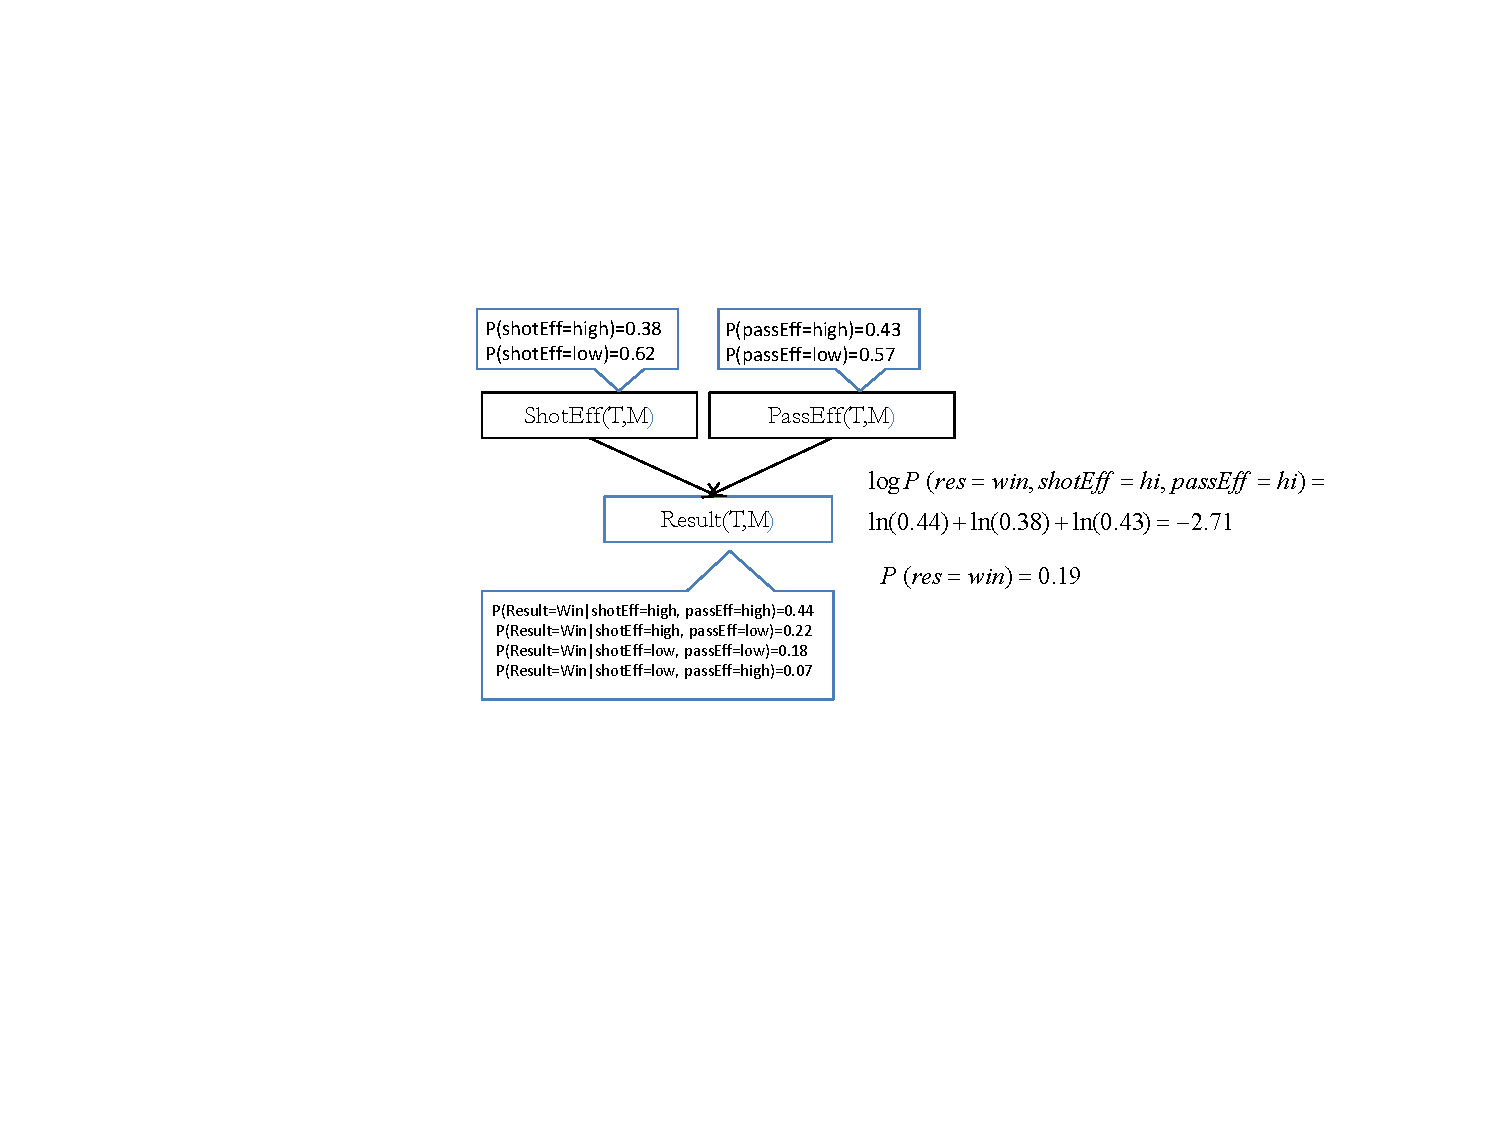
\includegraphics[width=0.4\textwidth] {BNExample.pdf}
	\caption{Example of joint and marginal probabilities computed from a toy Bayesian network structure. The parameters were estimated from the  Premier League dataset.
		%We show only the Markov blanket of the Results node to simplify. 
		\label{fig:bns}}
\end{figure}

\subsection{Relational Data}


 %We adopt the PBN formalism, following Poole's presentation.

%We apply the learn-and-join algorithm (LAJ), which is the state-of-the-art Bayes net learning method for relational data. The LAJ algorithm takes as input a relational database and outputs a Bayes net using the functor notation due to Poole \cite{Poole2003}. We briefly review this notation.

%\paragraph{Functor Terms} 
A functor is a function or predicate symbol. Each functor has a set of values (constants) called the \textbf{domain} of the functor. The domain of a \textbf{predicate} is $\{\true,\false\}$. A predicate of arity at least two is a \textbf{relationship} functor. Relationship functors specify which objects are linked. Other functors represent \textbf{features} or \textbf{attributes} of an object or a tuple of objects (i.e., of a relationship).
A \textbf{population} is a set of objects. 
A \textbf{term} is of the form $f(\term_{1},\ldots,\term_{k})$ where $\functor$ is a functor %(either a function symbol or a predicate symbol) 
and each $\term_{i}$ is a first-order variable or a constant denoting an object. A term is \textbf{ground} if it contains no first-order variables; otherwise it is a first-order term. In the context of a statistical model, we refer to first-order terms as \textbf{Parametrized Random Variables} (PRVs) \cite{Kimmig2014}. 
%A term whose range are the truth values $\{\true,\false\}$ is a \textbf{predicate}. 
%Predicates are usually written with uppercase Roman letters, other term with lowercase letters.
%The grounding concept represents moving from the population-level  to the object level. 
A \textbf{grounding} replaces each first-order variable in a term by a constant; the result is a ground term. A grounding may be applied simultaneously to a set of terms.  A relational database $\D$ specifies the values of all ground terms, which can be represented by data tables. 
%In machine learning terminology, the data tables are contingency tables that represent sufficient statistics or event counts.

Consider a joint assignment 
$P(\Features = \set{\nodevalue})$ of values to a set of PRVs $\Features$. The {\em grounding space} of the PRVs is the set of all possible grounding substitutions, each applied to all PRVs in $\Features$. The {\em count} of groundings that satisfy the assignment with respect to a database $\D$ is denoted by $\grounds_{\D}(\Features = \set{\nodevalue})$. The \textbf{database frequency} $P_{\D}(\Features = \set{\nodevalue})$ is the grounding count divided by the number of all possible groundings, that is, the size of the grounding space.
		
\emph{Example.} \label{sec:example}
%
The Opta dataset represents information about premier league data %\cite{opta-original} 
(Sec.~\ref{sec:real-world-data}). 
%Using the functor notation, the data
%format can be represented as follows. 
The basic populations are teams, players, matches, with 
corresponding first-order variables $\team, \player, \match$. Table~\ref{table:data} specifies values for some ground terms. Table~\ref{table:counts} illustrates grounding counts. Counts are based on the 2011-2012 Premier League Season. We count only groundings $(\it{team},\it{match})$ such that $\it{team}$ plays in $\it{match}$. Each team, including Wigan Athletics, appears in 38 matches. The total number of team-match pairs is $38 \times 20 = 760$.

%Examples of terms include the following. 

%\begin{itemize}
%\item $\it{Appears\_Player}(\P,\M)$ indicates whether a player appeared in a match.
%\item $\it{Appears\_Team}(\T,\M)$ indicates whether a team played in a match.
%\item $\it{Team}(\P)$ returns the team of a player.
%\item $\it{Result}(\T,\M)$ denotes the result of a team in a match (win or lose).
%\item $\it{ShotEff}(\T,\M)$ denotes the shot efficiency of a team in a match (number of successful shots on target, per total number of shots).
%\item $\it{TimePlayed}(\P,\M)$ denotes the total time that a player played in a match.
%\end{itemize}


%\begin{table}[htbp]
%\caption{Examples of terms in the soccer dataset.}
%\centering
%\resizebox{0.5\textwidth}{!}{
%\begin{tabular}{|c|p{5cm}|}
%\hline
%Term&Meaning\\ \hline
%$\it{Appears\_Player}(\P,\M)$ & indicates whether a player appeared in a match.\\ \hline
%$\it{Appears\_Team}(\T,\M)$&indicates whether a team played in a match.\\ \hline
%$\it{Team}(\P)$& returns the team of a player.\\ \hline
%$\it{Result}(\T,\M)$ &denotes the result of a team in a match (win or lose).\\ \hline
%$\it{ShotEff}(\T,\M)$ &denotes the shot efficiency of a team in a match (number of successful shots on target, per total number of shots).\\ \hline
%$\it{TimePlayed}(\P,\M)$& denotes the total time that a player played in a match.\\ \hline
%\end{tabular}}
%\label{table:terms}
%\end{table}

\begin{table}[htbp]
\caption{Sample Population Data Table (Soccer). The first three column headers show first-order variables for different populations. The remaining columns represent features.\label{table:data}}
\centering
\resizebox{0.5\textwidth}{!}{
\begin{tabular}{|c|c|l|c|c|c|c|}
\hline
 \multicolumn{1}{|l|}{MatchId \match} &
 TeamId \team & PlayerId \player& \multicolumn{1}{l|}{First\_goal(\player,\match)} 
& \multicolumn{1}{l|}{TimePlayed(\player,\match)} & 
\multicolumn{1}{l|}{ShotEff(\team,\match)}&result(\team,\match) \\ \hline
 117 & WA & McCarthy & 0 & 90 & 0.53&\it{win}\\ \hline
 147 & WA & McCarthy & 0 & 90 & 0.35&\it{loss}\\ \hline
 148 & WA & McCarthy & 0 & 85 & 0.57&\it{loss}\\ \hline
 15 & MC & Silva & 1 & 90 & 0.59&\it{win}\\ \hline
 175 & MC & Silva & 0 & 90 & 0.61&\it{win}\\ \hline
  \ldots& \ldots &\ldots&\ldots&\ldots&\ldots&\\
\end{tabular}}
\caption{Sample Object Data Table, for team $\team = \it{WA}$. \label{table:individual}}
\resizebox{0.5\textwidth}{!}{
\begin{tabular}{|c|c|l|c|c|c|c|}
\hline
 \multicolumn{1}{|l|}{MatchId \match} &
 TeamId $\team = \it{WA}$ & PlayerId \player& \multicolumn{1}{l|}{First\_goal(\player,\match)} 
& \multicolumn{1}{l|}{TimePlayed(\player,\match)} & 
\multicolumn{1}{l|}{ShotEff(\it{WA},\match)}&result(\it{WA},\match) \\ \hline
 117 & WA & McCarthy & 0 & 90 & 0.53&\it{win}\\ \hline
 147 & WA & McCarthy & 0 & 90 & 0.35&\it{loss}\\ \hline
 148 & WA & McCarthy & 0 & 85 & 0.57&\it{loss}\\ \hline
   \ldots& WA &\ldots&\ldots&\ldots&\ldots&\\
\end{tabular}}
\end{table}

A novel aspect of our paper is that we learn model parameters for specific objects as well as for the entire population. 
%To implement this, for each target object, we form 
The appropriate \textbf{object data table} is formed from the population data table by restricting the relevant first-order variable to the target object. 
For example, the object database for target Team $\it{Wigan Athletic}$, 
forms a subtable of the data table of Table~\ref{table:data} that contains only rows where 
TeamID = $\it{WA}$; see Table~\ref{table:individual}.

%\begin{table} 
%	\captionsetup{singlelinecheck=off}
%			\caption[.]{\label{table:counts}Example of Grounding Count and Frequency for the conjunction \begin{displaymath} \it{passEff(T,M)=hi}, shotEff(T,M)=high, Result(T,M)=1.\end{displaymath}}
%			\centering
%			\resizebox{0.5\textwidth}{!}{
%				\begin{tabular}{|c|c|c|}
%					\hline
%					Database&Count or $\#_{D}(\Features = \set{\nodevalue})$&Frequency or $P_{D}(\Features = \set{\nodevalue})$\\\hline
%					Population&76& $76/760=0.10$\\\hline
%					Wigan Athletics&7&$7/38=0.18$\\\hline
%		
%					%Synthetic&40&280\\ \hline
%				\end{tabular}}
%			\end{table}
\begin{table} 
	\caption{Example of Grounding Count and Frequency for the conjunction $\it{passEff(T,M)=hi}, shotEff(T,M)=high, Result(T,M)=1.$.\label{table:counts}}
	\centering
	\resizebox{0.5\textwidth}{!}{
		\begin{tabular}{|c|c|c|}
			\hline
			Database&Count or $\#_{D}(\Features = \set{\nodevalue})$&Frequency or $P_{D}(\Features = \set{\nodevalue})$\\\hline
			Population&76& $76/760=0.10$\\\hline
			Wigan Athletics&7&$7/38=0.18$\\\hline
			
			%Synthetic&40&280\\ \hline
		\end{tabular}}
	\end{table}

%\begin{table} 
%	\captionsetup{singlelinecheck=off}
%			\caption[.]{\label{table:counts}Example of Grounding Count and Frequency for the conjunction \begin{displaymath} \it{passEff(T,M)=hi}, shotEff(T,M)=high, Result(T,M)=1.\end{displaymath} Counts are based on the 2011-2012 Premier League Season. We count only groundings $(\it{team},\it{match})$ such that $\it{team}$ plays in $\it{match}$. Each team, including Wigan Athletics, appears in 38 matches. The total number of team-match pairs is $38 \times 20 = 760$.
%			\label{MetricComputation}}
%			\centering
%			\resizebox{0.5\textwidth}{!}{
%				\begin{tabular}{|c|c|c|}
%					\hline
%					Database&Count or $\#_{D}(\Features = \set{\nodevalue})$&Frequency or $P_{D}(\Features = \set{\nodevalue})$\\\hline
%					Population&76& $76/760=0.10$\\\hline
%					Wigan Athletics&7&$7/38=0.18$\\\hline
%		
%					%Synthetic&40&280\\ \hline
%				\end{tabular}}
%				
%			\end{table}
			
%[Example of counts, frequencies]
% For simplicity only, suppose that the only matches and players in the season are those shown in Table~\ref{table:data}. Then the attribute value $\it{First\_goals} = 0$ occurs with frequency $1/2$ in the object distribution $P_{\it{si}}$ for Silca. In the player class distribution $P_{\it{Player}}$, the attribute value $\it{First\_goals} = 0$ occurs with frequency $4/5$. So Silva is somewhat less likely to score no goal than a randomly selected player.
\subsection{Bayesian Networks for Relational Data}

A \textbf{Parametrized Bayesian Network Structure} (PBN) is a Bayesian network structure  whose nodes are PRVs. For most of the paper we refer to PBNs simply as Bayesian networks, and to PRVs simply as random variables. 
%The learn-and-join algorithm is the state-of-the-art Bayes net learning method for relational data, based on model search in the lattice of relationship joins \cite{Schulte2012}. The LAJ algorithm takes as input a relational database and outputs a Parametrized Bayes net structure.
%We review the algorithm very briefly; for further details please see \cite{Schulte2012}. 
%The algorithm builds a Bayes net for an entire database by level-wise search through the {\em lattice of relationship chains.} This is the lattice of relationship sets that are connected by shared first-order variables.
%%; see Figure~\ref{fig:lattice}.  
%%We describe the fundamental ideas of the algorithm; for further details please see \cite{Schulte2012}. 
%The user chooses a single-table Bayes net learner. The learner is applied to base population data tables. Then the learner is applied to data tables for relationship chains of size $s,s+1,\ldots$, with the constraint that the models for larger join tables inherit the absence or presence of learned edges from smaller join tables. 
%
The relationships and features in an object database define a set of nodes for Bayes net learning.  Figure~\ref{fig:bns} shows a sample PBN.


%We use the following notation.

%\begin{figure}[ht]
%\centering
%   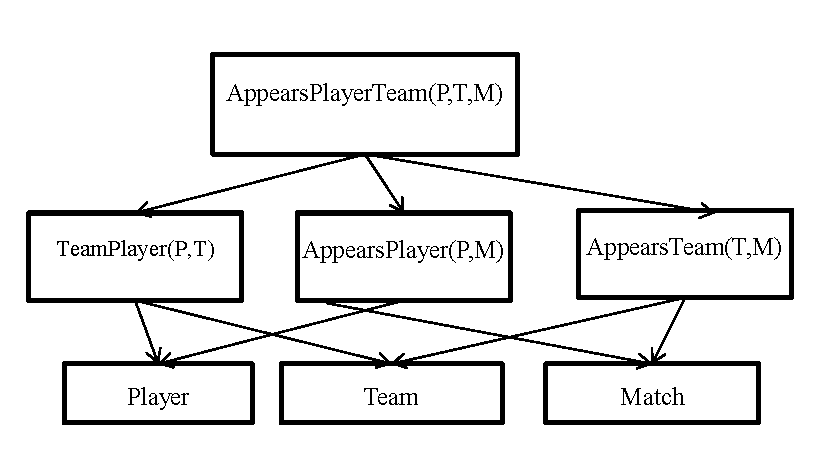
\includegraphics[width=0.3\textwidth] {lattice}
% \caption{Lattice of Premier League dataset.
% %We show only the Markov blanket of the Results node to simplify. 
% \label{fig:lattice}}
%\end{figure}




%\begin{itemize}
%\item $\D_{\population}$ is the database for the entire population; cf. Table~\ref{table:data}.
%\item $\D_{\target}$ is the restriction of the input database to the target object; cf. Table~\ref{table:object}. 
%\item $\M_{\population}$ is a model (e.g., Bayesian network) learned with $\D_{\population}$ as the input database; cf. Figure~\ref{fig:bns}(a).
%\item $\M_{\target}$ is an object model (e.g., Bayesian network) learned with $\D_{\target}$ as the input database; cf. Figure~\ref{fig:bns}(b).
%\end{itemize}
%

\subsubsection{Model Likelihood for Parametrized Bayesian Networks}

A standard method for applying a generative model assumes that the generative model represents normal behavior since it was learned from the entire population. An object is deemed an outlier if the model assigns sufficiently low likelihood to generating its features \cite{Cansado2008}. This likelihood method is an important baseline for our investigation.
%, so we define the likelihood function formally in this section. 
%The other outlier scores we consider can be viewed as improved variants of the likelihood approach. 
Defining a likelihood for relational data is more complicated than for i.i.d. data, because an object is characterized not only by a feature vector, but by an object  database.
% that lists the object's links and the attributes of linked entities. 
%For the model likelihood function $\lnlikelihood(\model,\D)$, where $\model$ denotes a Bayesian network, 
We employ the relational pseudo log-likelihood \cite{Schulte2011}, which can be computed as follows for a given Bayesian network  and database.

%\begin{eqnarray}
%\lnlikelihood(\model,\D) =   \sum_{i=1}^{n}\sum_{j=1}^{\states_{i}} \sum_{\parents_{i}}\\ P_{\D}(\feature_{i} = \nodevalue_{ij},\parents_{i})\ln \parameter_{\model}(\feature_{i} = \nodevalue_{ij}|\parents_{i})  \nonumber
%\end{eqnarray}

\begin{equation} \label{eq:likelihood}
\loglikelihood(\D,\model,\parameters) =   \sum_{i=1}^{n}\sum_{j=1}^{\states_{i}} \sum_{\parents_{i}}\P_{\D}(\nodevalue_{ij},\parents_{i})\ln \parameter(\nodevalue_{ij}|\parents_{i})  
\end{equation}


Equation~\ref{eq:likelihood} represents the standard BN log-likelihood function for the object profile data, except that parent-child instantiation counts are standardized to be proportions \cite{Schulte2012}. The equation can be read as follows.

\begin{enumerate}
\item For each parent-child configuration, 
use the maximum-likelihood estimate of the conditional probability of the child given the parent.
\item Multiply the logarithm of this estimate by the instantiation proportion of the parent-child configuration. The instantiation proportion is the number of instantiating groundings, divided by the total number of possible instantiations.
\item Sum this product over all parent-child configurations and all nodes. 
\end{enumerate}

%\begin{eqnarray}
%\lnlikelihood&   \sum_{i=1}^{n}\sum_{j=1}^{\states_{i}} \sum_{\parents_{i}} P_{\D}(\feature_{i} = \nodevalue_{ij},\parents_{i})\ln \parameter_{\model}(\feature_{i} = \nodevalue_{ij}|\parents_{i})
%\end{eqnarray}


{\em Example.} The family configuration \begin{displaymath} \it{passEff(T,M)=hi}, shotEff(T,M)=high, Result(T,M)=1\end{displaymath} contributes one term to the pseudo log-likelihood for the BN of Figure~\ref{fig:bns}. For the population database, this term is $0.1 \times \ln(0.44) =-0.08 $. For the  Wigan Athletics database, the term is $0.18 \times \ln(0.44) =-0.14 $. 
%consider the parent-child configuration as shown in Figure~\ref{fig:bns}(b). Suppose that the data show that team $\it{WA}$ played 20 matches  in formation 1 with team shot efficiency at level 2 and won 12 of these. Then the maximum likelihood estimate of winning given the parent values is $12/20=0.6.$ The instantiation count is 10, so the instantiation proportion is $10/20 =0.5$. This parent-child configuration contributes $\ln 0.5 \cdot 0.6 = -0.415$ to the aggregate pseudo-likelihood. 

%\section{Class and Object Distributions} 



%\section{Overview} We describe the object-oriented data model and our approach to defining an object outlier score. In the object-oriented data model, complex objects are composed of simpler objects. This can be visualized as a tree. Objects are associated with attribute values. In this paper we assume that attributes take on discrete values, but this is not essential for our approach. 
%Figure~\ref{fig:oobn} shows a typical object tree. Matches are complex objects containing a home team and an away team. The match result is a match attribute. Teams are complex objects comprising players. Some player attributes  depend on the context of the match. Players have a special attribute that specifies their class. Note that the same object can appear in different nodes (e.g., Van Persie). 
%
%\begin{figure*}[htbp]
%	\centering
%	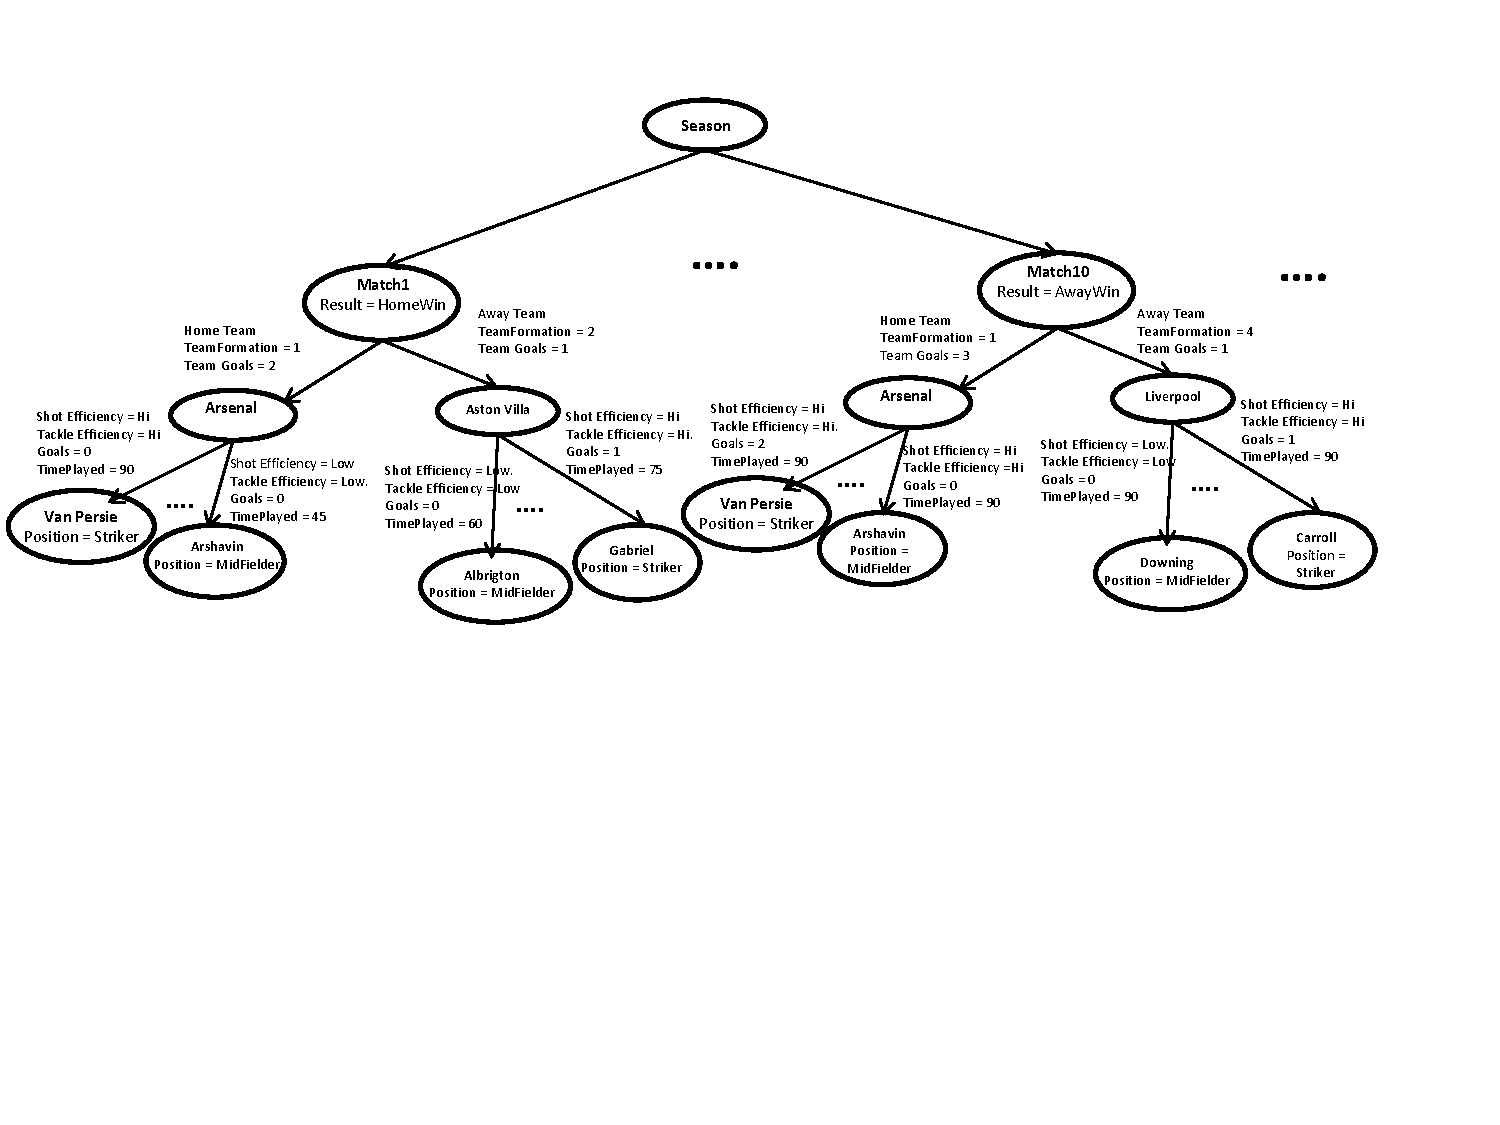
\includegraphics[width=1\textwidth]{SeasonGraph}
%	\caption{An illustrative object tree. Nodes are labelled with object IDs and object attributes. A season is a complex object comprising matches. A match comprises a home team and an away team. Teams comprise players. Edges go to component objects.  Edge labels indicate the type of component relationship between the linked objects, and attributes associated with this  relationship. 
%		\label{fig:oobn}}
%\end{figure*}
%
%Our system employs the following steps for outlier detection, illustrated in Figure~\ref{fig:}. 
%
%\begin{enumerate}
%	\item Define a set of path types in the object tree.
%	\item For a given target object, there is a substructure that contains the other objects linked to the target by paths of the applicable types. We refer to this substructure as the {\em object profile}.
%	\item For each attribute, the {\em object distribution} counts how many times the attribute occurred in the object's profile. 
%	\item We define a novel distribution divergence that measures how much the target object's distribution differs from the average distribution of objects in the same class. This divergence is our outlier score.
%\end{enumerate}
%
%In database terminology, an object profile is like a view centered on the object. For example, a query for computing the object profile for Arsenal would include the selection condition $\it{TeamID} = \it{Arsenal}$. Note that an object profile features both parts of the object as well as more complex objects of which it is a part. The object profile is individual-centered in the sense of \cite{Flach1999a}.
%
%\begin{figure}[htbp]
%	\centering
%	\resizebox{0.5\textwidth}{!}{
%		\includegraphics%[width=0.3\textwidth] 
%		{SystemOverView}
%	}
%	\caption{The components in our outlier detection system and the system flow. Aggregation is an alternative to our expected log-distance outlier score.
%		\label{fig:flow}}
%\end{figure}
%
%\section{Path Types}
%A path in the tree connects two nodes, with {\em links in either direction}. For example, the object tree contains a path $\it{van Persie} \leftarrow \it{Arsenal} \leftarrow \it{Match1}$ that connects van Persie to the first match of the season. Every path specifies a set of attribute values for the objects and edges contained in the path. 
%A \textbf{path type} is a set of paths with matching node types and matching edge types. For example, the path $\it{van Persie} \leftarrow \it{Arsenal} \leftarrow \it{Match10}$ is of the same type as the previous one.  For each attribute of a path type, and each value of the attribute, there is a count of the number of times that the attribute value occurs in a path of the type. These counts define the {\em path type distribution.} 
%%Given a list of path types, we can combine (concatenate) their distributions into a attribute distribution for the list. 
%%maybe use the term ``metapath''
%
%Assume that a list of path types have been fixed. The \textbf{object profile} contains all instances of a type of path that begin with the object. For each type of path, there is a distribution of attribute values over paths of that type in the object profile.
%The \textbf{object distribution} $P_{\object}$ for object $\object$ combines (concatenates) the path distributions 
%%over all attributes 
%in the object profile. 
%%In order words, it represents the distribution of attribute values over all paths that begin with the object.
%%a node labelled with the object's ID.
%The expression $P_{\Class}$ denotes the joint \textbf{class distribution} for the class of object $\object$. This is the joint probability associated with selecting an object uniformly at random from its class. Equivalently, the class distribution can be viewed as the  uniform mixture of object distributions:
%
%$$P_{\Class} \equiv \frac{1}{|\Class|} \sum_{\object \in \Class} P_{\object}.$$
%
%\paragraph{Example} Suppose we consider only paths of the type $\,$
%$\it{Player} \leftarrow 
%\it{Team} \leftarrow \it{Match}$. The attributes of this path type include $\it{Goals},\it{TeamGoals},\it{ShotEfficiency},\it{Result}$. For simplicity only, suppose that the only matches and players in the season are those shown in Figure~\ref{fig:oobn}. Then the attribute value $\it{Goals} = 0$ occurs with frequency $1/2$ in the object distribution $P_{\it{vP}}$ for van Persie. In the player class distribution $P_{\it{Player}}$, the attribute value $\it{Goals} = 0$ occurs with frequency $5/8$. So van Persie is somewhat less likely to score no goal than a randomly selected player.
%
%Since our outlier scores are based on the object profiles, they depend on a specification of relevant path types. One option would be to exhaustively include all possible path types. Another is to let a user specify path types of interest, for example all paths of length $k$. In our experiments we use machine learning methods that search the space of path types to find the paths that carry the strongest probabilistic associations between objects (see Section~\ref{sec:bnlearning}  below). 



%\section{Log-Distance Object Outlier score} \label{sec:metrics}
%%[There is no bound on the number of objects that a complex object may contain. ]
%
%[log distances. Motivation: additive, decomposed, closed form for computation. Relates to baseline methods. Distance not difference: avoid cancelling. Weight by frequency in object domain]
%
%Our approach defines an object-oriented outlier score as a {\em model comparison score} of the form 
%$$\scorediff(\model_{\object},\model_{\Class},\profile_{\object}).$$ Here $\profile_{\object}$ denotes the probability distribution defined by the profile of the potential outlier object $\object$, the symbol $\model_{\object}$ denotes a model of the object profile, and $\model_{\Class}$ denotes a model that represents the normal behavior in the population, learned from the entire dataset. 
%We use the following notation and definitions to define model comparison scores formally. %
%%\subsection{Notation and Bayesian Networks}
%Fix a set of attributes $\Features = \{\feature_{1},\ldots,\feature_{n}\}$. These are attributes of objects, which can and typically do belong to different classes. In statistical terms, each attribute defines a random variable. The possible values of $\feature_{i}$ are enumerated as $\{\nodevalue_{i1},\ldots,\nodevalue_{i\states_{i}}\}$. The notation $P(\feature_{i} = \x)\equiv P(\x)$ denotes the probability of attribute $\feature_{i}$ taking on value $\x$. We also use the vector notation $P(\Features = \set{x}) \equiv P(\set{x})$ to denote the joint probability of that each attribute $\feature_{i}$ takes on value $\set{x}_{i}$. 

\section{Likelihood-Distance Object Outlier score} \label{sec:metrics}

We introduce a novel model-based outlier score, that extends the log-likelihood, using the following notation.
\begin{itemize}
\item $\D_{\Class}$ is the database for the entire class of objects; cf. Table~\ref{table:data}. This database defines the \textbf{class distribution} $P_{\Class} \equiv P_{\D_{\class}}$.
\item $\D_{\object}$ is the restriction of the input database to the target object; cf. Table~\ref{table:individual}. This database defines the \textbf{object distribution} $P_{\object} \equiv P_{\D_{\object}}$.
\item $\model_{\Class}$ is a model (e.g., Bayesian network) learned with $\D_{\population}$ as the input database; cf. Figure~\ref{fig:bns}(a).
\item $\parameters_{\Class}$ resp. $\parameters_{\object}$ are parameters learned for $\model_{\Class}$ using $\D_{\class}$ resp. $\D_{\object}$ as the input database.
\end{itemize}

Figure~\ref{fig:flow} illustrates these concepts and the system flow for computing an outlier score. First, we learn a Bayesian network $\model_{\Class}$ for the entire population using a previous learning algorithm (see Section~\ref{sec:bnlearning} below). We then evaluate {\em how well the class model fits the target object.} The standard approach for vectorial data is to compute the log-likelihood of the class model for the target datapoint. Adapting this for relational data, we would compute the log-likelihood of the class model for the target  database:

\begin{equation} \label{eq:loglikelihood-score}
\loglikelihood(\D_{\object},\model_{\Class},\parameters_{\Class}).
\end{equation}

\begin{figure}
\centering
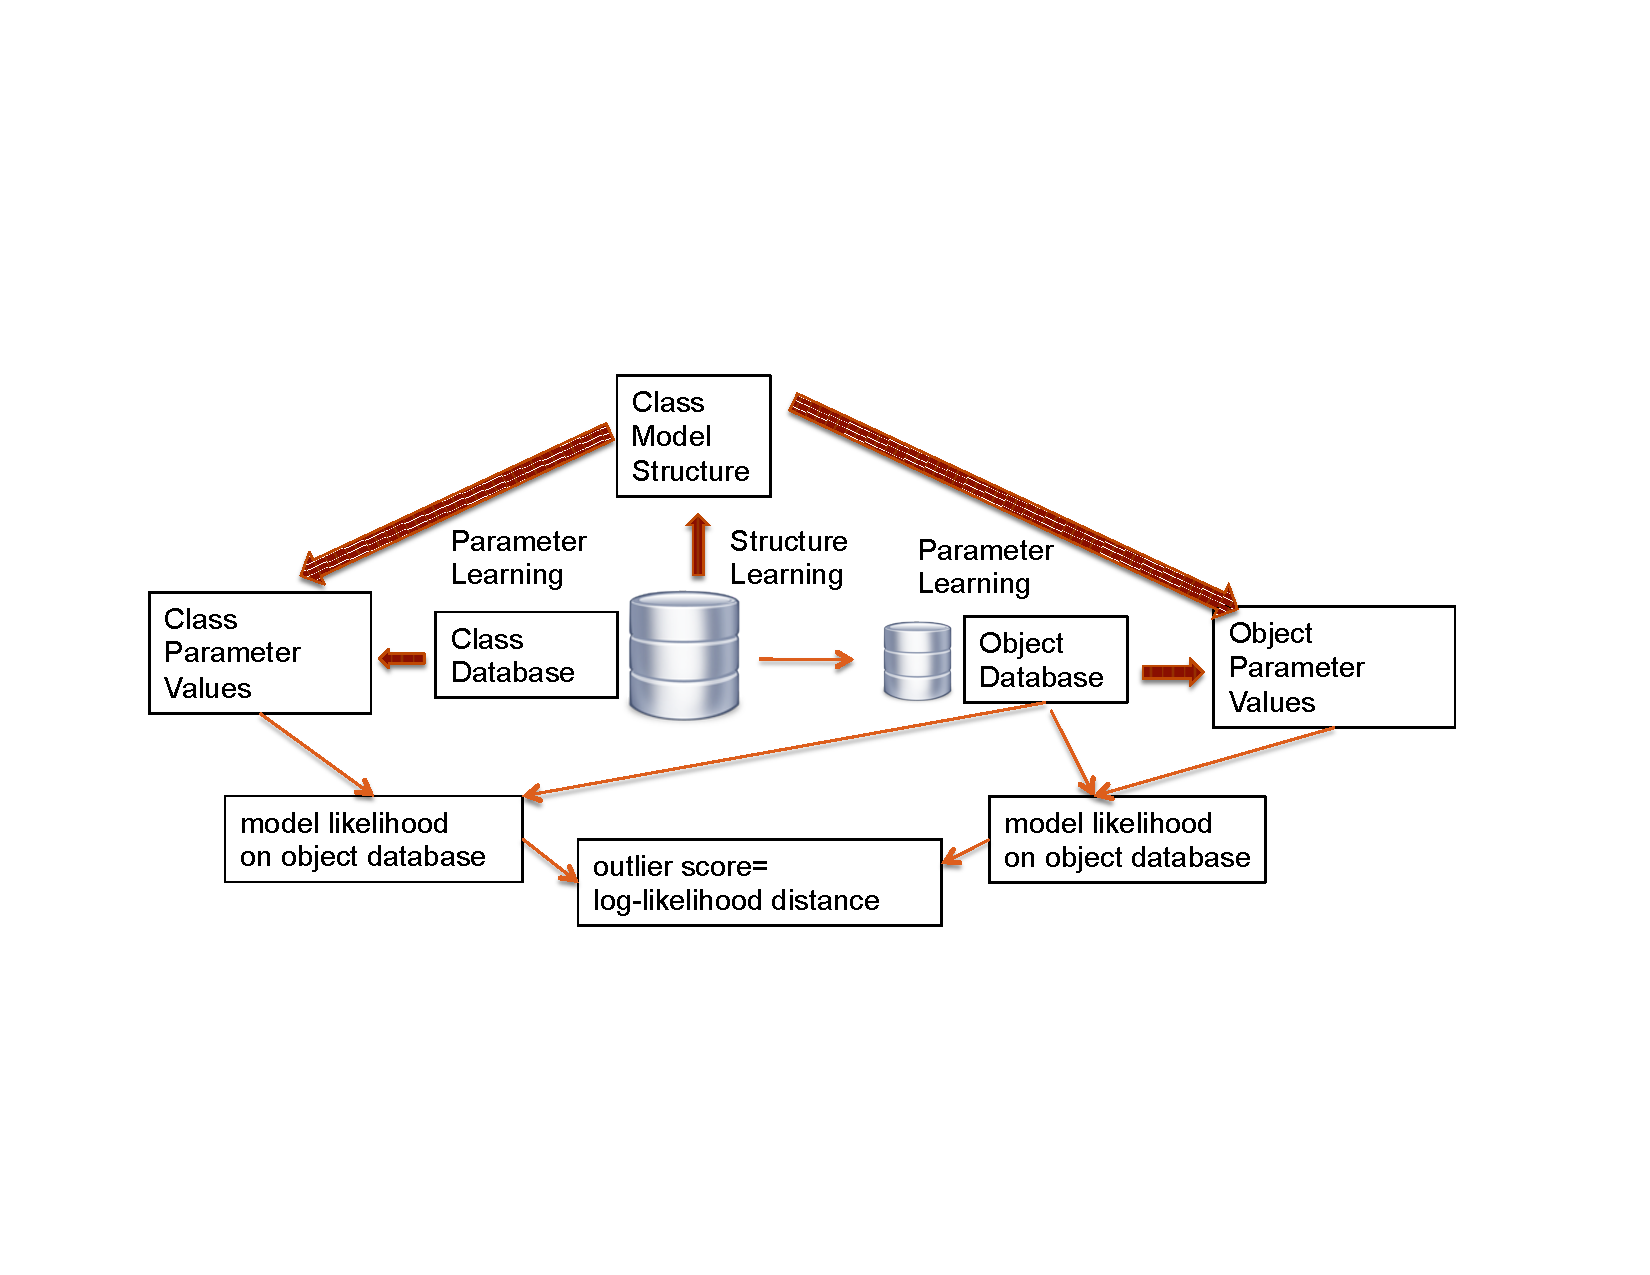
\includegraphics[width=0.5\textwidth]{flow.pdf}
\caption{Computation of outlier score.
\label{fig:flow}}
\end{figure}



While the log-likelihood~\eqref{eq:loglikelihood-score} is a good baseline outlier score, it is possible to improve further by considering scores based on the likelihood ratio, or {\bf log-likelihood difference}. The log-likelihood difference is defined by

\begin{equation} \label{eq:log-diff}
\loglikelihood(\D_{\object},\model_{\Class},\parameters_{\object}) - \loglikelihood(\D_{\object},\model_{\Class},\parameters_{\Class}).
\end{equation}

The log-likelihood difference compares  how well the class-level parameters fit the object profile, vs. how well the object parameters fit the object profile. In terms of the conditional probability parameters, the difference score measures how much the log-conditional probabilities in the class distribution differ from those in the object distribution. Note that this definition applies only for relational data where an individual is characterized by a substructure rather than a ``flat'' feature vector. Assuming maximum likelihood estimation, $\lr$ is equivalent to the Kullback-Leibler divergence between the class-level and object-level parameters~\cite{Campos2006}. 
%
While the difference score provides more outlier information than the model log-likelihood, it can be improved further by two transformations as follows. (1) Decompose the joint probability into a single-feature component and a mutual information component. (2) Replace log-likelihood differences by log-likelihood distances. The resulting score is the \textbf{log-likelihood distance} ($\mid$), which is the main novel score we propose in this paper. Formally it is defined as follows for each feature $i$. The total score is the sum of feature-wise scores. Section~\ref{sec:divergence-examples} below provides example computations.
%In other words, we assume that model comparison scores are decomposable, which is the case for Bayesian networks. 
%\small
%\begin{equation} \label{eq:mid-bn}
%\begin{aligned}
%%\sum_{j=1}^{\states_{i} P_{\object}(\feature_{i} = \nodevalue_{ij}) \left|\ln \frac{P_{\object}(\feature_{i} = \nodevalue_{ij})}\right| + \\
%%\sum_{i=1}^{n} \sum_{j=1}^{\states_{i}}P_{\object}(\feature_{i}=\nodevalue_{ij}) \ln \frac{P_{\object}(\feature_{i} = \nodevalue_{ij})}{P_{\Class}(\feature_{i} = \nodevalue_{ij})} +\\
%\mid_{i} =\sum_{j=1}^{\states_{i}} P_{\object}(\feature_{i} = \nodevalue_{ij}) \left|\ln \frac{P_{\object}(\feature_{i} = \nodevalue_{ij})}{P_{\Class}(\feature_{i} = \nodevalue_{ij})}\right|+\\
%\sum_{j=1}^{\states_{i}} \sum_{\parents_{i}} 
%P_{\object}(\feature_{i} = \nodevalue_{ij},\parents_{i})\\
%\left|\ln \frac{P_{\object}(\feature_{i} = \nodevalue_{ij}|\parents_{i})}{P_{\object}(\feature_{i})=\nodevalue_{ij}} - \ln \frac{P_{\Class}(\feature_{i} = \nodevalue_{ij}|\parents_{i})}{P_{\Class}(\feature_{i})=\nodevalue_{ij}}\right|.
%\end{aligned}
%\end{equation}
%\normalsize

%\small
\begin{equation} \label{eq:log-dist}
\begin{array}{l}
 %\sum_{j=1}^{\states_{i} P_{\object}(\feature_{i} = \nodevalue_{ij}) \left|\ln \frac{P_{\object}(\feature_{i} = \nodevalue_{ij})}\right| + \\
		%\sum_{i=1}^{n} \sum_{j=1}^{\states_{i}}P_{\object}(\feature_{i}=\nodevalue_{ij}) \ln \frac{P_{\object}(\feature_{i} = \nodevalue_{ij})}{P_{\Class}(\feature_{i} = \nodevalue_{ij})} +\\
		\mid_{i} =\sum_{j=1}^{\states_{i}} P_{\object}(\nodevalue_{ij}) \left|\ln \frac{\parameter_{\object}( \nodevalue_{ij})}{\parameter_{\Class}( \nodevalue_{ij})}\right|+\\
		\sum_{j=1}^{\states_{i}} \sum_{\parents_{i}} 
		P_{\object}( \nodevalue_{ij},\parents_{i})
		\left|\ln \frac{\parameter_{\object}( \nodevalue_{ij}|\parents_{i})}{\parameter_{\object}(\nodevalue_{ij})} - \ln \frac{\parameter_{\Class}( \nodevalue_{ij}|\parents_{i})}{\parameter_{\Class}(\nodevalue_{ij})}\right|. \end{array}
		\end{equation}
		%\normalsize
%\paragraph{Motivation} 
%
%We note that for a fixed object distribution $P_{\object}$, the log-likelihood distance is a proper distance metric between the class-level and the object-level parameters. 
%The $\mid$ has two components. 
The first sum is the \textbf{single-feature} component, where each feature is considered independently of all others. It computes the expected log-distance with respect to  the singe feature value probabilities between the object and the class models. 
%For example, the single-feature sum for the feature ``Goal" of Van Persie is 5/8. 
%
The second $\mid$ sum is the \textbf{mutual information component}, based on the mutual information among all feature. It computes the expected log-distance between the object and the class models with respect to the mutual information of feature value assignments.
%measures the expected distance in 
%%{\em multi-variate mutual information} 
%{\em association component} between the object and the class distributions. 
Intuitively, the first sum measures how the models differ if we treat each feature in isolation. The second sum measures how the models differ in terms of how strongly the features are associated with each other. 
%A standard result in information theory states that a joint distribution can, without loss of information, be decomposed into a univariate distribution and the multi-variate mutual information  \cite{Witten2005}. Considering how the distributions differ in each of these two terms therefore involves no loss of information. 

%$\mid$ is not symmetric between the object and the class distribution because it weights sum terms by the joint probability in  the object distribution. The lack of symmetry is a desirable feature because to assess whether an object is an outlier, we want to weight most the events that occur more frequently with the object. 

\subsection{Motivation} 
%The motivation for using log-distances %rather than log-differences 
%is that some log-differences are positive, some negative, and cancel each other out when their sign differs. Since our goal is to assess the distinctness of an object, {\em we do not want differences to cancel out.} Fundamentally, averaging differences is appropriate when considering costs, payoffs or utilities, but not appropriate when assessing the distinctness of an object. 
%
The motivation for the mutual information decomposition is two-fold. (1) {\em Interpretability}, which is very important for outlier detection. The single-feature components are easy to interpret since they involve no feature interactions. Each multi-feature local factor is based on the relevance of a small set of parent conditions for predicting the value of the child node, of the form $\ln \parameter(\nodevalue_{ij}|\parents_{i})/\parameter(\nodevalue_{ij})$ . This relevance term  is basically the same as the widely used lift measure \cite{Tuffery2011}, therefore an intuitively meaningful quantity. The $\mid$ score compares how relevant a given parent condition is in the object profile with how relevant it is in the general class. (2) {\em Avoiding cancellations.} The log-likelihood ratio decomposes into a relevance difference and a marginal difference: 

\begin{equation} \label{eq:decompose}
\ln \frac{\parameter_{\object}( \nodevalue_{ij}|\parents_{i})}{\parameter_{\Class}( \nodevalue_{ij}|\parents_{i})} = \ln \frac{\parameter_{\object}(\nodevalue_{ij}|\parents_{i})}{\parameter_{\object}(\nodevalue_{ij})} - \ln \frac{\parameter_{\Class}( \nodevalue_{ij}|\parents_{i})}{\parameter_{\Class}(\nodevalue_{ij})} + \ln \frac{\parameter_{\object}( \nodevalue_{ij})}{\parameter_{\Class}( \nodevalue_{ij})}.
\end{equation}

These differences can have different signs for different child-parent configurations and cancel each other out. Taking distances as in Equation~\ref{eq:log-dist} avoids this undesirable cancellation. Since our goal is to assess the distinctness of an object, {\em we do not want differences to cancel out.} Averaging differences is appropriate when considering costs, payoffs or utilities, but not appropriate when assessing the distinctness of an object. 



\subsection{Comparison Outlier Scores} Our lesion study compares our log-likelihood distance  $\mid$ score to baselines that are defined by omitting a component of $\mid$. In this section we define these scores  and provide a theoretical comparison. The scores increase in sophistication in the sense that they apply more transformations of the log-likelihood ratio. 
%Our empirical comparison below indicates that the 
More sophisticated scores provide more information about outliers.   
%defines the scores formally.  
Table~\ref{table:Formula} defines local feature scores; the total score is the sum of feature-wise scores. All metrics are defined such that {\em a higher score indicates a greater anomaly.} The metrics are as follows. 

\begin{LaTeXdescription}
\item[Feature Divergence $\fd$] is the first  component of the $\mid$ score. It considers each feature independently (no feature correlations).
%							
\item[Log-Likelihood Score \loglikelihood] is the standard model-based outlier detection score.
\item[Log-Likelihood Difference \lr] is the log-likelihood difference between the class-level and object-level parameters (Equation~\ref{eq:log-diff}). 
\item[Log-Likelihood Difference with absolute value $|\lr|$] replaces differences in $\lr$ by distances.
\item[Log-Likelihood Difference with decomposition $|\lr^{+}|$] applies a mutual information decomposition to $\lr$.
\end{LaTeXdescription}



	\begin{table}
		\caption{Baseline Outlier Scores for Bayesian Networks
			\label{table:Formula}}
		\resizebox{0.5\textwidth}{!}{
			\begin{tabular}{|l|l|} \hline
					Method & Formula\\
					\hline
				
							$\fd_{i}	$&	$\begin{array}{l}\sum_{i=1}^{n}\sum_{j=1}^{\states_{i}} P_{\object}( \nodevalue_{ij}) \left|\ln \frac{\parameter_{\object}( \nodevalue_{ij})}{\parameter_{\Class}( \nodevalue_{ij})}\right|\end{array}	$\\ \hline
						
						$-\loglikelihood_{i}$& $  \begin{array}{l} -\sum_{i=1}^{n}\sum_{j=1}^{\states_{i}} \sum_{\parents_{i}} P_{\object}( \nodevalue_{ij},\parents_{i})\ln \parameter_{\Class}( \nodevalue_{ij}|\parents_{i})\end{array}$ \\ \hline
					$\lr_{i}$&$\begin{array}{l}  \sum_{j=1}^{\states_{i}} \sum_{\parents_{i}} P_{\object}( \nodevalue_{ij},\parents_{i})\ln \frac{\theta_{\object}(  \nodevalue_{ij}|\parents_{i})}{\theta_{\Class}( \nodevalue_{ij}|\parents_{i})}.  \end{array}$\\	\hline
					$|\lr_{i}|$& $\begin{array}{l}  \sum_{j=1}^{\states_{i}} \sum_{\parents_{i}} P_{\object}( \nodevalue_{ij},\parents_{i})|\ln \frac{\theta_{\object}(\nodevalue_{ij}|\parents_{i})}{\theta_{\Class}( \nodevalue_{ij}|\parents_{i})}|. \end{array}$ \\	\hline
					$\lr_{i}^{+}$&$\begin{array}{l}  \sum_{j=1}^{\states_{i}} P_{\object}( \nodevalue_{ij}) \ln \frac{\parameter_{\object}( \nodevalue_{ij})}{\parameter_{\Class}( \nodevalue_{ij})}+
					\\ \sum_{j=1}^{\states_{i}} \sum_{\parents_{i}} 
					P_{\object}( \nodevalue_{ij},\parents_{i})
					\ln \frac{\theta_{\object}( \nodevalue_{ij}|\parents_{i})}{\parameter_{\object}(\nodevalue_{ij})} - \ln \frac{\theta_{\Class}( \nodevalue_{ij}|\parents_{i})}{\parameter_{\Class}(\nodevalue_{ij})}.  \end{array}$ \\ \hline
				
			\end{tabular} 
		}
	\end{table}


%Comparing Equations~\eqref{eq:lr+} and~\eqref{eq:mid-bn} we see that the $\mid$ score is obtained from the $\lr^{+}$ score by using absolute values of differences (in our notation, $\mid = |\lr^{+}|$. A standard result in information theory states that a joint distribution can, without loss of information, be decomposed into a univariate distribution and the multi-variate mutual information. This implies that the decomposed KLD score $\lr^{+}$ is identical to $\lr$. 
%the distinction between $\lr$ and $\mid$ is as follows: $\lr$ computes the expected log-{\em differences}, whereas $\mid$ computes the expected log-{\em distances}. Many standard divergence measures for distributions \cite{Chan2004} compute expected differences; we argue that for outlier detection, {\em one should compute expected distances instead.} The fundamental reason is that averaging differences is appropriate when considering costs, payoffs or utilities, but not appropriate when assessing the distinctness of an object. For example, $\lr$ can be interpreted as the average difference in message length when data points are encoded following the class distribution rather than the object distribution \cite{Tuffery2011}.
%\cite{Witten2005}. 
%If we treat message length as a cost, then $\lr$ computes the average cost of using the class distribution rather than the object distribution. 
%Some message lengths are shorter in the class distribution, some in the object distribution, and these differences cancel out. Since our goal is to assess the distinctness of an object, {\em we do not want differences to cancel out.}

%The next proposition shows that the outlier scores have the standard properties of a divergence measure between probability distributions: they are nonnegative, and 0 if and only if the class and object distributions are the same. Also, the triangle inequality entails that the scores can be ordered by dominance: one is guaranteed to be at least as great as another. Dominance means that a divergence potentially provides more discrimination among objects as it maps the set of objects onto a larger range of scores. Our $\mid$ score dominates all others.  We provide empirical evidence that dominance does correspond to greater discrimination.
%
%\begin{mydef} Assume maximum likelihood estimation for the object-level parameters $\parameters_{\object}$. Then for any class and object distribution, we have $\mid \geq |\lr| \geq \lr = \lr^{+} \geq 0$. The outlier scores are 0 if and only if the the object and class distribution are the same; otherwise, all inequalities are strict.
%\end{mydef}
%
%{\em Proof Outline.} The inequalities all follow from the triangle inequality $|a|+|b|\geq |a+b|$. The equality $\lr = \lr^{+}$ follows by applying the decomposition~\ref{eq:decompose}. The maximum likelihood parameters maximize the function $\loglikelihood(\D_{\object},\model_{\Class},\cdot)$ \cite{Schulte2012}, so the log-likelihood ratio $\lr$ is positive if and only if $\theta_{\Class} = \theta_{\parameters}$.
%\vspace{-5mm}
%\paragraph{Computational Complexity} Assume that for each joint assignment of values $\set{x}$, the object probability $P_{\object}(\set{x})$ and the class probabilities $P_{\class}(\set{x})$ can be computed in linear time (e.g., by a table lookup). Then the computational complexity of evaluating the $\mid$ score is bounded by the number of joint assignments $\prod_{i=1}^{n} \states_{i}$. This term grows exponentially with the number of attributes. In the next section we discuss how the computational cost of evaluating the score can be greatly reduced by employing a Bayesian network representation of the class and object distributions. 



%\section{Bayesian Network Representation}\label{sec:bn}
%
%
%
%
%
%Given a BN representation of the object and class distribution, the $\mid$ score is computed as follows: 
%
%$\begin{array}{l} 
%%\sum_{j=1}^{\states_{i} P_{\object}(\feature_{i} = \nodevalue_{ij}) \left|\ln \frac{P_{\object}(\feature_{i} = \nodevalue_{ij})}\right| + \\
%%\sum_{i=1}^{n} \sum_{j=1}^{\states_{i}}P_{\object}(\feature_{i}=\nodevalue_{ij}) \ln \frac{P_{\object}(\feature_{i} = \nodevalue_{ij})}{P_{\Class}(\feature_{i} = \nodevalue_{ij})} +\\
%\mid =\sum_{j=1}^{\states_{i}} \parameter_{\object}( \nodevalue_{ij}) \left|\ln \frac{P_{\object}( \nodevalue_{ij})}{\parameter_{\Class}( \nodevalue_{ij})}\right|+\\
%\sum_{i=1}^{n}\sum_{j=1}^{\states_{i}} \sum_{\parents_{i}} 
%P_{\object}( \nodevalue_{ij},\parents_{i})
%\left|\ln \frac{\parameter_{\object}( \nodevalue_{ij}|\parents_{i})}{\parameter_{\object}(\nodevalue_{ij})} - \ln \frac{\parameter_{\Class}( \nodevalue_{ij}|\parents_{i})}{\parameter_{\Class}(\nodevalue_{ij})}\right|.
%\end{array}$
%
%We emphasize that Equation~\eqref{eq:mid-bn} is not a new outlier score compared to Equation~\eqref{eq:mid}. It is the same score using the Bayesian network factorization~\eqref{eq:bn} of the $\mid$ divergence~\eqref{eq:mid}. We derive Equation~\ref{eq:mid-bn} by starting with the BN expression of the KL divergence \cite{Neapolitan2004}, then apply the mutual information decomposition as in Equation~\ref{eq:kld-transform}, finally average log-distances rather than log-differences.  
%%\vspace{-5mm}
%\paragraph{Motivation} It is well-known that compared to a flat table representation of a joint distribution, the factored BN representation~\eqref{eq:bn} can be and typically is exponentially smaller \cite{Pearl1988}. Our experiments show this compression effect empirically  (Table~\ref{table:Number of Parameters}). With the BN representation, the $\mid$ score can be computed in time and space cost linear in the number of the conditional probability parameters in the object and class BNs. This typically provides an exponential reduction in computation cost compared to the tabular representation~\eqref{eq:mid}. 
%
%
%%Since the score decomposes into a sum, we can easily find the local factors that have the highest impact on it. This means that the $\mid$ score provides a kind of {\em subspace analysis.} Subspace analysis aims to find ascertain which subset of attributes contributes the most to a given outlier score. A standard approach searches for attribute subsets that are irrelevant in that eliminating them makes little difference to the outlier ranking. As our case study in the following illustrates, the BN metric supports finding the attributes with the most impact on the outlier score without the need for searching the space of attribute subsets. 
%
%In addition to compactness, another advantage of the BN representation is {\em interpretability}. Interpretability is very important for outlier detection. The BN form of the $\mid$ score is easily interpreted because it {\em decomposes} into a sum of {\em local} factors. Each multi-attribute local factor is based on the relevance of a small set of parent conditions for predicting the value of the child node. This relevance term is basically the same as the widely used lift measure \cite{Tuffery2011}, therefore an intuitively meaningful quantity. The $\mid$ score compares how relevant a given parent condition is in the object profile with how relevant it is in the general class. 
%the conditional probability parameters correspond to {\em local} features that describe the conditional distribution of a single variable given a fairly small set of parent values. 
%The Bayes net advantages of compactness and interpretability carry over to the $\mid$ score, as 




%Since the score decomposes into a sum, we can easily find the local factors that have the highest impact on it. This means that the $\mid$ score provides a kind of {\em subspace analysis.} Subspace analysis aims to find ascertain which subset of attributes contributes the most to a given outlier score. A standard approach searches for attribute subsets that are irrelevant in that eliminating them makes little difference to the outlier ranking. As our case study in the following illustrates, the BN metric supports finding the attributes with the most impact on the outlier score without the need for searching the space of attribute subsets. 
%
%In our experiments we use Bayesian networks to represent the joint distributions for an object and its class. Our outlier metrics can also be defined in terms of generic joint distributions, without assuming that the distributions are represented by a Bayesian network. Our experiments use Bayesian network representations as well, so the formulas we present show the computations used in our evaluation.

%
% Using Bayesian networks to represent joint distribution has two key advantages \cite{Pearl1988}. (1) Compactness: the number of conditional probabilities that need to be specified is typically much less than the total number of joint probabilities. 
%% For instance, if the BN contains $n$ binary nodes, there are $2^{n}$ joint probabilities. If each node has a relatively small number $k$ of parents (a typical maximum is $k=5$), the number of parameters is only $n \cdot 2^{k}$, basically linear compared to the full set of $2^{n}$ numbers for specifying the joint probabilities directly. 
% %
% (2) Interpretability: the conditional probability parameters correspond to {\em local} attributes that describe the conditional distribution of a single variable given a fairly small set of parent values. The Bayes net advantages of compactness and interpretability carry over to object-oriented outlier metrics, which we discuss next.
%
\begin{figure*}[htbp]
	\centering
	\resizebox{0.85\textwidth}{!}{
		\includegraphics%[width=0.3\textwidth] 
		{figures/figure1kddCropped.pdf}
	}
	\caption{Illustrative Bayesian networks. The networks are not learned from data, but hand-constructed to be plausible for the soccer domain. (a) High Correlation: Normal individuals exhibit a strong association between their features, outliers no association. Both normals and outliers have a close to uniform distribution over single features.
		% The outlier distribution misses a correlation that is present in the normal population. The single feature distributions are uniform in both distributions. 
		(b) Low Correlation: Normal individuals exhibit no association between their features, outliers have a strong association. Both normals and outliers have a close to uniform distribution over single features.
		% The outlier object exhibits a correlation that is not present in the normal population. The single attribute distributions are uniform in both distributions.
		(c) Single Attributes: Both normal and outlier individuals exhibit a strong association between their features. In normals, 50\% of the time, feature 1 has value 0. For outliers, feature 1 has value 0 only 10\% of the time. 
		%Correlations are the same, but the single feature distributions are not.
		\label{fig:synthetic-bns}}
\end{figure*}


\section{Examples} \label{sec:divergence-examples} 


We provide three simple examples with only two features that illustrate the computation of the divergences. They are designed so that outliers and normal objects are easy to distinguish, and so that it is easy to trace the behavior of an outlier score.
%The examples also illustrate the concepts of attribute and correlation outlier. 
The examples therefore serve as thought experiments that bring out the strengths and weaknesses of probabilistic divergences when used for object outlier detection. 
Figure~\ref{fig:synthetic-bns} describes the BN representation of the examples. Table~\ref{table:example} provides the computation of the divergences.
% 
The table illustrates the undesirable cancelling effects in $\lr$. In the high correlation scenario~\ref{fig:synthetic-bns}(a), the outlier object has a lower probability than the normal class distribution of $\it{Match\_Result} = 0$ given that $\it{Shot\_Efficiency} = 1$. Specifically, 0.5 vs. 0.9. The outlier object exhibits a higher probability $\it{Match\_Result} = 1$ than the normal class distribution, conditional on $\it{Shot\_Efficiency} = 1$; specifically, 0.5 vs. 0.1. In line 1, column 2 of Table~\ref{table:example}  the log-ratios $\ln(0.5/0.9)$ and $\ln(0.5/0.1)$ therefore have different signs. In the low correlation scenario~\ref{fig:synthetic-bns}(b), the cancelling occurs in the same way, but with the normal and outlier probabilities reversed. 
%The cancelling effect is even stronger for attributes with more than two possible values.


\begin{table}[hbpt]
	\caption{Computation of different outlier divergences for the example distributions of Figure~\ref{fig:synthetic-bns}(a),(b). Divergences for the $F_{2}$ feature are computed conditional on $F_{1} = 1$. Expectation terms are computed first for $F_{2} = 1$, then $F_{2} = 0$. The single feature distributions are uniform, so the feature component $\mid_{1}$ 
		is 0 for each node in both examples. } \label{table:example}
	
	%\captionsetup[table]{skip=10pt}
	
	\centering
	\resizebox{0.5\textwidth}{!}{
		\begin{tabular}{|c|p{3cm}|p{6cm}|l|}
			\hline
			Score&$F1=1$ Computation&$F2|F1=1$ Computation&Result\\ \hline
			$\lr$&\begin{tabular}{p{5cm}} $1/2 \ln(0.5/0.5)=0 $\end{tabular}&$1/4\ln(0.5/0.9)+ 1/4\ln(0.5/0.1)$&0.36\\ \hline
			%$ELD$&$1/2|\ln(0.5/0.5)|=0$&$1/4|\ln(0.5/0.9)|+1/4|\ln(0.5/0.1)|$&0.79\\ \hline
			$|\lr|$&$0$ (no parents)&\begin{tabular}{p{5cm}}$1/4 |\ln(0.5/0.5)-\ln(0.9/0.5)|+1/4 |\ln(0.5/0.5)-\ln(0.1/0.5)|$\end{tabular}&0.79\\ \hline
			$\fd$&$|\ln(0.5/0.5)|=0$&\begin{tabular}{p{5.5cm}}$1/2|\ln(0.5/0.5)| + 1/2|\ln(0.5/0.5)|$\end{tabular}&0\\ \hline
			$$\mid$$&$0+0$&$0.79+0$&0.79
			%$1/4(|\ln(0.9/0.5)-\ln(0.5/0.5)|+|\ln(0.1/0.5)-\ln(0.5/0.5)|+2|\ln(0.5/0.5)|)=0.54$
			\\ \hline
		\end{tabular}}
		%\centering
		\resizebox{0.5\textwidth}{!}{
			\begin{tabular}{p{8cm}}
				\textbf{Table V(a): High Correlation: The divergences for the object and class BNs of Figure~\ref{fig:synthetic-bns}(a).}
			\end{tabular}}
			
			%
			\centering
			\resizebox{0.5\textwidth}{!}{
				\begin{tabular}{|l|p{3cm}|p{6cm}|l|}
					\hline
					Score&$F1=1$ Computation&$F2|F1=1$ Computation&Result\\ \hline
					$\lr$&$1/2\ln(0.5/0.5)=0$&$0.5 \cdot 0.9 \ln(0.9/0.5)+ 0.5 \cdot 0.1 \ln(0.1/0.5)$&0.26\\ \hline
					%$ELD$&$1/2|\ln(0.5/0.5)=0|$&$0.5 \cdot 0.9|\ln(0.9/0.5)|+0.5 \cdot 0.1|\ln(0.1/0.5)|$&0.50\\ \hline
					$|\lr|$&$0$ (no parents) &$0.5 \cdot 0.9 |\ln(0.9/0.5)-\ln(0.5/0.5)|+ 0.5 \cdot 0.1 |\ln(0.1/0.5)-\ln(0.5/0.5)| $&0.50\\ \hline
					$\fd$&$|\ln(0.5/0.5)|=0$&$1/2|\ln(0.5/0.5)| + 1/2|\ln(0.5/0.5)|$&0\\ \hline
					$\mid$&$0+0$&$0.5+0$&0.5\\ \hline
				\end{tabular}}
				\resizebox{0.5\textwidth}{!}{
					\begin{tabular}{p{8cm}}
						\textbf{Table V(b): Low Correlation: The divergences for the object and class BNs of Figure~\ref{fig:synthetic-bns}(b). }
					\end{tabular}}
				\end{table}
				
				
				
				
				
				%The advantages of succinctness and interpretability obtain also for computing divergences. We write $B_{\object}$ for a BN that represents the object distribution, and $B_{\Class}$ for a BN that represents the class distribution. Then $\lr$ can be decomposed as $\lr = \sum_{i =1} ^{n} \lr_{i}$, where $$\lr_{i} = \sum_{j=1}^{\states_{i}} \sum_{\parents_{i}} \ln \frac{P_{B_{\object}}(\feature_{i} = \nodevalue_{ij}|\parents_{i})}{P_{B_{\Class}}(\feature_{i} = \nodevalue_{ij}|\parents_{i})}$$ where $\parents_{i}$ indexes all possible parent value combinations for node $\feature_{i}$, and the $P_{B}$ terms denote the conditional probability parameters of the applicable Bayesian network. In words, we sum over all possible child-parent states, and compute the log-probability ratio of the object and class conditional probabilities. The Bayesian network decompositions for the other divergences are as follows. We compute feature divergence as before directly from the class and object distributions, rather than the Bayesian networks, since it concerns only marginal single-feature probabilities. 
				
				%\begin{eqnarray*} 
				%%\tag{$\lr(P_{\object}||P_{\Class})$} 
				%\eld_{i} & = & \sum_{j=1}^{\states_{i}} \sum_{\parents_{i}} |\ln \frac{P_{B_{\object}}(\feature_{i} = \nodevalue_{ij}|\parents_{i})}{P_{B_{\Class}}(\feature_{i} = \nodevalue_{ij}|\parents_{i})}|\\
				%\jid_{i} & = & \sum_{j=1}^{\states_{i}} \sum_{\parents_{i}} |\ln \frac{P_{B_{\object}}(\feature_{i} = \nodevalue_{ij}|\parents_{i})}{P_{\object}(\feature_{i})=\nodevalue_{ij}} - \ln \frac{P_{B_{\Class}}(\feature_{i} = \nodevalue_{ij}|\parents_{i})}{P_{\Class}(\feature_{i})=\nodevalue_{ij}}|\\
				%\mid_{i} & = &
				%\label{eq:eld}
				%\end{eqnarray*}
				
				
				
				
				
								%The learning algorithms were executed with 64-bit Centos with 4GB RAM and an Intel Core i5-480 M processor. 
				
				
				
				%\subsection{Outlier Metrics Compared}
				
				%\begin{description} 
				%We evaluate the outlier divergences $\mid,\eld,\lr$ described in Section~\ref{sec:divergences}. 
				%
				%We use two existing baseline methods. 
				
				%\paragraph{Likelihood Method.} 
				%The metric $\lnlikelihood$ is defined by the equation:
				
				%\begin{equation*} \label{eq:ll}
				%\lnlikelihood_{i} = \sum_{j=1}^{\states_{i}} \sum_{\parents_{i}} P_{\object}(\feature_{i} = \nodevalue_{ij},%\parents_{i})\ln P_{\Class}(\feature_{i} = \nodevalue_{ij}|\parents_{i})
				%\end{equation*}
				
				%The intuition behind this metric is that the class distribution Bayesian network represents normal behavior\cite%{riahi2013}. An object is deemed an outlier if  the class BN assigns sufficiently low likelihood to generating %its features. Using low model likelihood to identify outliers is a common application of Bayesian networks \cite%{Cansado2008a}.  The equation above represents the standard BN log-likelihood function for the object data, %except that parent-child instantiation counts are standardized to be proportions. 
				%This avoids giving exponentially more influence to features with more groundings \cite{Schulte2011}. 
				
				
				%\item[\mid] The outlier metric is the Mutual Information Distance defined in Equation \eqref{eq:mid}. 
				%
				%\item[\eld] The outlier metric is the Mutual Information Distance defined in Equation \eqref{eq:eld}. 
				%
				%\item[\lr] The outlier metric is the KL divergence between the generic and the individual feature distribution. 
				%
				%\item[\lnlikelihood]  The outlier metric is the standardized log-likelihood $\lnlikelihood$ of the generic Bayesian network applied to the individual feature distribution. 
				%\marginpar{define, ranks everything the same on BN example (b).}
				%\item[\lr] The outlier metric is the likelihood ratio metric $\lr$. The Bayesian network learning method for the target individual's network uses the LAJ algorithm.
				
				%\item[
				
				%\paragraph{Local Outlier Factor.}
				
				%The local outlier factor is a popular density-based outlier metric that has been used as a baseline in previous %studies \cite{Breunig2000}. The metric requires specifying the number of nearest neighbors $k$. The authors of %the $\lof$ method recommend choosing a value between 10 and 20; we use 10 and 20.
				%\end{description}
				
				%$\lof$ requires as input a flat data matrix where each individual is represented by a single feature vector. To %aggregate features of individuals across complex objects such as matches or ratings, we use the total feature %count. This is the approach of the inventors of $\lof$ for sports data \cite{Breunig2000}. For example, they %counted the total number of goals scored by a player in a season as a feature for outlier analysis. We used the %implementation of $\lof$ in $\it{Data mining with R(DMwR)}$ package in R.
				
				%\subsection{Performance Metric} To score each outlier metric against ground truth instances, we follow the %%%approach of \cite{Gao2010,Cansado2008a}: Given the ground truth that $r\%$ of instances are outliers, we sort the outlier scores in descending order, and take the top $r\%$ as the outliers indicated by the method. We then report the true positive rate (recall), or \textbf{true outlier rate} (TOR), and the true negative rate, or \textbf{true normal rate} (TNR). The TNR is thus the percentage of normal individuals with rank below the top $r\%$. In anomaly detection the true outlier rate is the most important metric \cite{Gao2010,Cansado2008a}.
				\section{Experimental Design}
Details about our systems and algorithms that we use from previous work may be found in Section~\ref{sec:details}.  
We begin with a description of the datasets that we have used in our experiments.
				
				\subsection{Synthetic Datasets}
				
				We generated three synthetic datasets with normal and outlier players using the distributions represented in the three Bayesian networks of Figure~\ref{fig:synthetic-bns}. 
				%The features $F_{1}$ and $F_{2}$ represent two features of players. 
				Each player participates in 38 matches, similar to the real-world data. The main goal of designing synthetic experiments is to test the methods on  easy to detect outliers. Each match assigns a value to each feature $F_i, i =  1,2$ for each player. 
				\begin{LaTeXdescription}
				\item\textbf{High Correlation} See Figure~\ref{fig:synthetic-bns}(a).
				\item\textbf{Low Correlation} See Figure~\ref{fig:synthetic-bns}(b).
				\item\textbf{Single features} See Figure~\ref{fig:synthetic-bns}(c).
				\end{LaTeXdescription}
			
				
				
				
				
				%These datasets are designed so that outliers and normal objects are easy to distinguish, and so that it is easy to trace the behavior of an outlier score.
				
				%\begin{description}
				%\item[High Correlation]  See Figure~\ref{fig:synthetic-bns}(a).
				%\item[Low Correlation]  See Figure~\ref{fig:synthetic-bns}(b).
				%\item[Single attributes] See Figure~\ref{fig:synthetic-bns}(c).
				%\end{description}
				%
				We used the $\it{mlbench}$ package in $\it{R}$ to generate synthetic features in matches, following these distributions for 240 normal players and 40 outliers. We followed the real-world Opta data in terms of number of normal and outlier individuals. The scores are used to rank all 280 players. 
				\subsection{Real-World Datasets} \label{sec:real-world-data}
				Data tables are prepared from Opta data~\cite{opta-original} and IMDb~\cite{IMDb-original}. Our datasets and code are available on-line~\cite{bib:jbnsite}. Table~\ref{table:Features} lists relationships and the number of features. 
				\begin{table}[htbp]
							\caption{Relationships and Features in Real-World Datasets.
								%For relationships please see text.
								\label{table:Features}}
					\centering
					\resizebox{0.4\textwidth}{!}{
						\begin{tabular}{|l|c|l|}
							\hline
							Path/Object Type & \#Attributes&Example\\ \hline
							\begin{tabular}{c}Player-Team-Match \end{tabular} & 11&ShotEff \\ \hline
							\begin{tabular}{c}Team-Match \end{tabular} & 7&TeamFormation \\ \hline\hline
							Actor & 2&Quality \\ \hline
							Director & 2&AvgRevenue\\ \hline
							Movie&5&Genre\\ \hline
							User& 2&Occupation\\ \hline
							User-Movie & 1&Rating \\\hline
							Actor-Movie & 1&Cast\_Position\\\hline
						\end{tabular}}
				
					\end{table}
					\begin{LaTeXdescription}
						\item[Soccer Data]
						The Opta data were released by Manchester City. 
						It lists all the ball actions within each game by each player, for the 2011-2012 season.
						\item[IMDb Data]
						The Internet Movie Database (IMDb) is an online database of information related to films, television programs, and video games.
						The IMDb website offers a dataset containing information on cast, crew, titles, technical details and biographies in a set of compressed text files \cite{Peralta2007}.
					\end{LaTeXdescription}
					
					%\subsection{Outlier and Contrast Classes.}
					
					In real-world data, there is no ground truth about which objects are outliers. To address this issue, we employ a one-class design: we learn a model for the class distribution, with data from that class only. Then we rank all individuals from the normal class together with all objects from a contrast class treated as outliers, to test whether an outlier score distinguishes objects from the normal class from objects in the contrast class. Table~\ref{MetricComputation} shows the normal and contrast classes for three different datasets.  In-class outliers are possible, e.g. unusual strikers may be members of the striker class. In case studies section we show a few in-class outliers. In the soccer data, we considered only individuals who played more than 5 matches. The maximum number of matches played is 38.
%
%					In this design, we are only looking for the objects that are clearly deviating from the majority of the data. We are aware of the 
					
										%
					%\begin{description}
					%\item[Strikers vs. Goalies] The generic model is learned with match data from all 150 strikers. The outlier test cases are match data for all 22 goalies.
					%\item[Midfielder vs. Striker]  The generic model is learned with match data from all 172 midfielders. The outlier test cases are match data for 70 randomly selected strikers.
					%\item[Drama vs. Comedy] The generic model is learned with data for all 400 drama movies and 80 randomly selected comedy movies.
					%\end{description}
					%Figure~\ref{fig:synthetic} shows the true outlier rates for the different outlier metrics.  {\em On all datasets, the Mutual Information Divergence $\mid$ separates the normal class from the contrast class better than the other methods.} The same is true for the true negative rate; see supplementary file.
					%This rate reflects only the number of contrast objects that are ranked highly. Therefore we cannot expect a true outlier rate of 100\% because the normal class may also contain genuine outliers. If a metric correctly ranks these within-class outliers more highly than contrast class members, its TOR decreases. 
					% that are not in the contrast some strikers, may be genuine outliers within the striker class.
					
					\begin{table}
							\caption{Outlier/normal Objects in Real-World Datasets. }
							\label{MetricComputation}
						\centering
						\resizebox{0.4\textwidth}{!}{
							\begin{tabular}{|c|c|c|c|}
								\hline
								Normal&\#Normal&Outlier&\#Outlier\\\hline
								Striker & 153 & Goalie&22\\ \hline
								Midfielder & 155 & Striker&74\\ \hline
								Drama & 197 & Comedy&47\\ \hline
								%Synthetic&40&280\\ \hline
							\end{tabular}}
						
						\end{table}
						
%						\subsection{Performance Score}
%					 Our experiments provide empirical evidence that $\mid$ works better than other scores for object outlier detection.
%						Our performance score for outlier rankings is the area under curve ($\auc$) of the well-established receiver operating characteristic $\roc$ curve.
%						~\cite{Fawcett2006}. 
%						This has been widely used to measure the performance of outlier ranking methods~\cite{Cansado2008, Muller2012}. The relationship between false positive rate (1- Specificity) and true positive rate (Sensitivity) is captured by the $\roc$ curve. Ideally, the best performance is achieved when we have the highest sensitivity and the highest specificity. 
%					
%						The maximum values for $\auc$ is 1.0 indicating a perfect ranking with 100\% sensitivity and 100\% specificity. In order to compute the $\auc$ value, we used the \textit{R} package \textit{ROCR}~\cite{RROCR2012}. Given a set of outlier scores, one for each object, this package returns an $\auc$ value. 
%					
																
						\subsection{Methods Compared}
						
						We compare two types of approaches, and within each approach several outlier detection methods. The first approach uses the likelihood-based outlier scores described in Section~\ref{sec:metrics}. For relational Bayesian network structure learning we use the previous state-of-the-art learn-and-join algorithm, described in the appendix (Section~\ref{sec:bnlearning}).
						
%						probabilistic scores applied directly to the  data structured as an object tree. 
						The second approach first ``flattens" the structured data into a matrix of feature vectors, then applies standard matrix-based outlier detection methods. We refer to such method as \textbf{aggregation-based}
						%Flattening the object data allows applying the rich set of matrix-based outlier detection methods ``as is" 
						(cf. Figures~\ref{fig:novelty}). For example, this was the approach taken by Breunig {\em et al.} for identifying anomalous players in sports data \cite{Breunig2000}. Following their paper, for each continuous feature in the object profile, we use the average over its values, and for each discrete feature, we use the occurrence count of each feature value in the object data. Aggregation 
						tends to lose information about correlations .
						%\cite{DavidJensen2002}. 
Our experiments evaluate the empirical question of whether this loss of information affects outlier detection. 
						%The advantage to the aggregation approach is that after aggregating to preprocess the data, any matrix-based outlier detection method can be applied; see Figure~\ref{fig:flow}. 
						We evaluated three standard matrix-based outlier detection methods.

						
						
						
						
					%	\subsubsection{Structured Data Methods}
						
%						These include the $\mid$ and $\lr$ scores 
%						that we introduced in Section~\ref{sec:metrics}. In addition, we apply the following two scores.
%						
%						
%						
%						 Including it as a baseline provides a lesion study for how important it is to consider the mutual information among attributes.
%						Low model likelihood is a common score for using Bayesian networks to identify outliers \cite{Cansado2008}. The intuition behind the $\lnlikelihood$ score is that the class distribution Bayesian network represents normal behavior~\cite{riahi2013}. Low model likelihood therefore indicates anomalous objects. This is a common score for using Bayesian networks to identify outliers \cite{Cansado2008}.
						%An object is deemed an outlier if  the class BN assigns sufficiently low likelihood to generating its attributes.  
%						The equation above represents the standard BN log-likelihood function for the object profile data, except that parent-child instantiation counts are standardized to be proportions \cite{Schulte2012}. 						
						%\subsubsection{Aggregation-based Matrix Methods}
						
						%%Standard outlier detection methods  require as input a flat data matrix where each individual is represented by a single attributes vector. To aggregate attributes of individuals across complex objects such as matches and ratings, we use the total attribute count. This is the approach that the inventors of $\lof$ \cite{Breunig2000} applied to sports data. For example they counted the total number of goals scored by a player in a season as a attribute for outlier analysis. 
%						
						%For example, in the soccer dataset there is a correlation between ``shot efficiency" and ``dribble efficiency" of a striker and that correlation is a key feature to identify strikers from other class. However when we use the averages of these attributes,
						%%, by averaging over all the values of continuous attributes and counting the number of occurrences of different states of discrete attributes in all the player's matches, 
						%the correlation no longer exists. 
												% for comparison with $\mid$.
						%assume that the observations comprise independent data points that can be represented in a matrix. Since 
						%
						%Then, we study performance of \textit{MID} metric in comparison with:
						%\begin{description}
						%\item[$\lof$] is a density-based method originally presented in~\cite{Breunig2000} as a measure to quantify the outlier-ness of the data points relative to regions of different densities. Therefore, the score is defined based on local density instead of the nearest neighbor distance. In the simple words, $\lof$ compares the density of area around an object to the densities of the areas of the surrounding objects. However, $\lof$ defines density as the inverse of the average of the smoothed reachability distances in a neighborhood and this definition is not the precise definition of density in terms of number of data points within a specific region. $\lof$ is only sensitive to the density of the area and  ignore the orientation and the shape of the area.
						%\item[$\outrank$] is a subspace outlier ranking technique that employs the subspace analysis to identify the degree of outlierness. It compares clustered regions in different subspace and derive the outlierness score for each object. In this work we used $\outrank$ with two subspace clustering models \textit{PRO-CLUS} \cite{Muller2009} and \textit{DISH} \cite{Kriegel2007} (as suggested in~\cite{Muller2012} \textit{PRO-CLUS} is the best clustering function for their approach).
						%\item[$\knn$] is a well-known distanced-based outlier ranking method that is based on the distance of a point from its $k^{th}$ nearest neighbor and rank each object on the basis of its $k^{th}$ nearest neighbor. \cite{Ramaswamy2000}.
						%\end{description}
						
						\begin{LaTeXdescription}
							\item[$\lof$] is a standard density-based method~\cite{Breunig2000}.
							%It quantify the outlier-ness of the data points relative to regions of different densities. Therefore, the score is defined based on local density instead of the nearest neighbor distance. In the simple words, 
							$\lof$ compares the density of area around an object to the densities of the areas of the surrounding objects. 
							%However, $\lof$ defines density as the inverse of the average of the smoothed reachability distances in a neighborhood and this definition is not the precise definition of density in terms of number of data points within a specific region. $\lof$ is only sensitive to the density of the area and  ignore the orientation and the shape of the area.
							\item[$\knn$] is a well-known distanced-based outlier ranking method that assigns a score to each data point on the basis of distance of the point from its $k^{th}$ nearest neighbor ($D^k$) and  declare the top $n$ points as outliers~\cite{Ramaswamy2000}. 
							%They introduce a {\em partition-based} algorithm to set a upper bound and lower bound on $D^k$ to identify the partitions that cannot contain the top $n$ outliers and prune them in order to limit the search space. % \textbf{Sarah:more precise please}
							\item[$\outrank$] employs subspace analysis to measure the degree of outlierness. It compares clusters in different subspace to derive an outlier score for each object \cite{Muller2012}. \end{LaTeXdescription}
						
						Density and distance based methods are two fundamental approaches to outlier detection represented in our study by $\lof$ and $\knn$. Subspace analysis is a popular approach too, and relevant to our study because $\mid$ is sensitive to correlations among features as well. 
						
						
						\section{Empirical Results}
						
						We present results regarding computational feasibility, 
						%$\auc$ 
						predictive performance, and case studies.
						
						\emph{Computational Cost of the ELD Score.}
%						
%						Table~\ref{table:Number of Parameters} shows that the Bayesian network representation provides a highly compact summary of the target class distribution: the number of probabilities that need to be evaluated for computing the probabilistic scores decreases by a factor of 
%						%\textbf{Sarah:fix dash}
%						$10^{4}$\--$10^{5}$ depending on the dataset. 
%						
						Table~\ref{table:LearningTime} shows that the computation of the $\mid$ value for a given target object is feasible. It takes a quarter of a minute for each soccer player, and one minute for each movie. This includes the time for BN learning. Learning the class-level BN takes longer, but needs to be done only once for the entire object class. The BN model is crucial for computational feasibility because it provides a compact low-dimensional representation of the joint distribution information in the data. Table~\ref{table:Number of Parameters} compares the number of terms required to compute the ELD score in the BN representation to computing it with a unfactored representation with one parameter for each joint probability.
						
						\begin{table}[htbp]
						
							\begin{subtable}
								%\caption{Time for computing the $\mid$ metric. This includes the time for Bayes Net structure learning.\label{table:LearningTime}}
								\centering
									\caption{Time for computing the $\mid$ score. This includes the time for Bayes Net structure learning.\label{table:LearningTime}}
								\resizebox{0.5\textwidth}{!}{
									\begin{tabular}{|c|l|l|} \hline
										Dataset& Class (min)
										%    \begin{tabular}{c} Class \\Terms (min)\end{tabular}   & 
										%    \begin{tabular}{c} Object \\Terms (min)\end{tabular}   
										& Object (min) \\ \hline
										Strikers vs. Goalies&4.14&0.25\\ \hline
										Midfielder vs. Goalies &4.02&0.25 \\ \hline
										Drama vs. Comedy &8.30&1.00\\ \hline
									\end{tabular} 
								}
							
							\end{subtable}

							\begin{subtable}
								%\caption{The Bayesian network representation helps to decrease the number of terms that represent the class and object distributions. 
								%For relationships please see text.
								%\label{table:Number of Parameters}}
								\centering
									\caption{The Bayesian network representation decreases the number of terms required for computing the $\mid$ score.
										%that represent the class and object distributions.
										\label{table:Number of Parameters}}
								\resizebox{0.5\textwidth}{!}{
									\begin{tabular}{|c|l|l|}
										\hline
										Dataset & \begin{tabular}{c} \#Terms \\Using BN\end{tabular}  & \begin{tabular}{c} \#Terms \\ without Using BN
										\end{tabular}\\ \hline
										Strikers vs. Goalies & 1,430&114,633,792\\ \hline
										Midfielders vs. Goalies & 1,376&43,670,016\\ \hline
										Drama vs. Comedy & 50,802&215,040,000\\ \hline
									\end{tabular}
								}
							
							\end{subtable}
							
													\end{table}
						
						\subsubsection{Detection Accuracy} We follow the evaluation design of~\cite{Gao2010} and 
	make each baseline methods detect the same percentage of  objects as outliers:
	% as that of the ground-truths. To achieve this, we 
					Sort the outlier scores obtained by the three baseline methods in descending order, and take the top $r$ percent as outliers. Then we use \textbf{precision}, a.k.a. \textbf{true positive rate} as the evaluation metric which is the percentage of correct ones in the set of outliers identified by the algorithm. As in ~\cite{Gao2010}, we set the percentages of outlier to be 5\% and 15\%.\footnote{We also applied other outlier detection metrics, such as AUC and recall, but omit the details due to space constraints. Our $\mid$ score performs the best with these other metrics as well, to a similar degree.} In the one-class design, precision measures how many members of the outlier class were correctly recognized.

						
						\paragraph{Likelihood-Based Methods} 
						
						
						Table~\ref{table:Method Comparison} shows the $\auc$ values for each probabilistic ranking. Our $\mid$ score achieves the best accuracy. On the synthetic data, it ought to be easy to distinguish the outliers, but {\em $\mid$ is the only score that achieves perfect detection}. %For this reason, in Table~\ref{table:Method Comparison} we compare only the performance of $\mid$ to the previous data matrix methods.
%						\begin{table}
%							\begin{subtable}
%								
%								\centering
%									\caption{$\auc$ of $\mid$ vs. other probabilistic scores. 
%										%For relationships please see text.
%										\label{table:Metric Comparison}}
%								\resizebox{0.5\textwidth}{!}{
%									
%									\begin{tabular}{|l|l|l|l|l|}
%										\hline
%										Dataset & \mid &\lr &\fd&\lnlikelihood\\ \hline
%										
%										Synthetic Data-High Correlation & \textbf{1.00}&0.95&0.88&0.98 \\ \hline
%										Synthetic Data-Low Correlation & \textbf{1.00}&0.95&0.35&0.95 \\ \hline
%										Synthetic Data-Single Feature & \textbf{1.00}&0.89&0.79&0.98 \\ \hline
%										Real Data-Strikers vs. Goalies & \textbf{0.89} &0.61&0.83& 0.65\\ \hline
%										Real Data-Midfielders vs. Strikers &\textbf{0.66} &0.64 &0.52&0.64 \\ \hline
%										Real Data-Drama vs. Comedy & \textbf{0.70} &0.65&0.61&0.63 \\ \hline
%									\end{tabular}}
%								
%								\end{subtable}
%								
%								\begin{subtable}
%									
%									\centering
%										\caption{$\auc$ of $\mid$ vs. aggregation-based Outlier Ranking Methods. 
%											%For relationships please see text.
%											\label{table:Method Comparison} 
%										}
%									\resizebox{0.5\textwidth}{!}{
%										\begin{tabular}{|l|c|c|c|c|c|}
%											\hline
%											Dataset & $\mid$ &$\lof$&\begin{tabular}{c}$\outrank$\\(ProClus)\end{tabular}&\begin{tabular}{c}$\outrank$\\(DISH)\end{tabular}&\begin{tabular}{c}\it{KNN}\\\it{Outlier}\end{tabular}\\ \hline
%											
%											High Correlation & \textbf{1.00}&0.87&0.73&0.95&0.92 \\ \hline
%											Low  Correlation & \textbf{1.00}&0.53&0.33&0.32&0.45 \\ \hline
%											Single Feature & \textbf{1.00}&0.58&1.00&0.96&0.95\\ \hline
%											Strikers vs. Goalies & \textbf{0.89} &0.68&0.89&0.53&0.75 \\ \hline
%											Midfielders vs. Strikers &\textbf{0.66} &0.53 &0.54&0.49&0.55 \\ \hline
%											Drama vs. Comedy & \textbf{0.70} &0.53&0.56&0.42&0.61 \\ \hline
%										\end{tabular}}
%									
%									\end{subtable}
%								\end{table}
%											\begin{table}
%									
%															\caption{Precision of $\mid$ compare to other baseline scores in different datasets
%																\label{table:CaseStudy}}
%															\resizebox{0.5\textwidth}{!}{	
%															\begin{tabular}{|l|c|c|c|c|c|c|c|c|}\hline
%																	Dataset&\multicolumn{5}{|c|}{Structured-based models }&\multicolumn{3}{|c|}{Aggregation-based models}\\
%																	\hline
%																 &\mid&$|KLD|$&\lr&\fd&\lnlikelihood&\lof&$\outrank$	&\knn\\
%																	\hline
%																	High-Correlation &\textbf{1.00}&\textbf{1.00}&0.85&0.65&0.95&0.22&0.50&0.65\\
%																	\hline	
%																	Low-Correlation&\textbf{1.00}&\textbf{1.00}&0.90&0.25&0.95&0.25&0.10&0.10\\
%																	\hline
%																	Single-Feature&\textbf{1.00}&\textbf{1.00}&0.55&0.62&0.92&0.55&1.00&0.67\\\hline
%																	Striker-Goali&\textbf{0.63}&0.36&0.31&0.58&0.40&0.32&0.50&0.52\\\hline
%																	Midfielder-Striker&\textbf{0.52}&0.50&0.39&0.44&0.50&0.38&0.48&0.35\\\hline
%																	Drama-Comedy&\textbf{0.47}&0.45&0.44&0.40&0.28&0.36&0.17&0.20\\\hline
%																\end{tabular}	}		
%																	
%												\end{table}
												
		\begin{table}
																																\caption{Precision of $\mid$ compared to other baseline scores in different datasets.
						\label{table:Method Comparison}}
												\resizebox{0.5\textwidth}{!}{	
												\begin{tabular}{|l|c|c|c|c|c|c|c|c|c|}\hline
													Dataset& precision&\multicolumn{5}{|c|}{Structured-based models }&\multicolumn{3}{|c|}{Aggregation-based models}\\
														\hline
																& &\mid&$|\lr|$&\lr&\fd&\loglikelihood&\lof&$\outrank$	&\knn\\
																	\hline
															    \multirow{2}{*}{High-Correlation}& 5\%& \textbf{1.00}& \textbf{1.00}& 0.73& 0.47& 0.91& 0.11& 0.53& 0.48\\
															    &15\%&\textbf{1.00}&\textbf{1.00}&0.85&0.65&0.95&0.22&0.50&0.65\\
														    \hline																				    	 \multirow{2}{*}{Low-Correlation}& 5\%& \textbf{1.00}& \textbf{1.00}& 0.87& 0.14& 0.93& 0.10& 0.00& 0.06\\
												    	    &15\%&\textbf{1.00}&\textbf{1.00}&0.90&0.25&0.95&0.25&0.10&0.14\\
													    	    \hline
																\multirow{2}{*}{Single-Feature}& 5\%& \textbf{1.00}& \textbf{1.00}& 0.39& 0.53& 0.81& 0.46& \textbf{1.00}& 0.51\\
															&15\%&\textbf{1.00}&\textbf{1.00}&0.55&0.62&0.92&0.55&\textbf{1.00}&0.54\\
															\hline    
																\multirow{2}{*}{Striker-Goali}& 5\%& \textbf{0.57}& 0.27& 0.22& 0.51& 0.36& 0.19& 0.47& 0.42\\
																	&15\%&\textbf{0.63}&0.36&0.31&0.58&0.40&0.32&0.50&0.52\\
																	\hline    
															\multirow{2}{*}{Midfielder-Striker}& 5\%&\textbf{ 0.49}& 0.42& 0.25& 0.41& 0.46& 0.29& 0.44& 0.16\\
															&15\%&\textbf{0.52}&0.48&0.39&0.44&0.50&0.38&0.48&0.35\\
												\hline  																				\multirow{2}{*}{Drama-Comedy}&5\%& \textbf{0.44}& 0.38& 0.39& 0.15& 0.22& 0.29& 0.07& 0.014\\
															&15\%&\textbf{0.47}&0.45&0.44&0.40&0.28&0.36&0.17&0.20\\
																\hline     
																					
												\end{tabular}	}		
																	
						\end{table}
								\paragraph{Aggregation-Based Methods vs. \mid} 
								Table~\ref{table:Method Comparison} shows the precision values for aggregation-based methods compared to $\mid$. {\em Our $\mid$ score outperforms all aggregation-based methods on all datasets}, except for a tie with $\outrank$(ProClus) on the relatively easy problem of distinguishing strikers from goalies.
%								Comparing tables~\ref{table:Metric Comparison} and~\ref{table:Method Comparison} shows that t
								The performances of aggregation-based methods are most like that of the probabilistic score $\fd$, which does not consider the
								correlation among the features. This finding reflects the fact that aggregation tends to lose information about correlations.
								% \cite{DavidJensen2002}. 
								The aggregation-based methods achieve their highest performance on the Strikers vs. Goalies dataset. In this dataset action count features such as ShotsOnTarget, ShotEfficiency point to strikers and the feature SavesMade points to goalies. Therefore, outliers in this dataset are also easy to find by considering features in isolation.
								%\\
								%\\
								%Based on the results shown in table ~\ref{table:Method Comparison}, the easiest dataset is Single Features, as most of the methods are successful in detecting outliers in that dataset. The low correlation dataset seems to be the most challenging one. 
								%The results of $\knn$ seem to be closest to $\mid$ in most datasets. 
								
								%The $\roc$ curve in Figure~\ref{fig:ROC} shows the performance of $\mid$ and $\knn$ which indicates that $\mid$ always reaches a higher true positive rate earlier that $\knn$.
								%\textbf{Sarah: both graph and table?}
								%Show the running time in a table. Explain that thats one of the weakness of $\mid$ compare to the others. But since the its performance is much higher than the compatitors it is worth the waiting!
								
								%
								%
								%
								%Strikers vs. goalies dataset is very similar to synthetic dataset, single feature in a sense that outlier and normal classes in both datasets contain single features that have distinct and very different distributions independent of the other attributes. In Strikers vs. Goalies attributes such as ShotsOnTarget or ShotEfficiency are valid only if the object is a member of Striker class and SavesMade only belongs to Goalie Class. Therefore, outliers in this dataset are also very easy to find even by applying the aggregation-based methods.  
								
								
								
								%\begin{figure*}
								%\centering
								%\resizebox{0.9\textwidth}{!}{
								
								%\subfigure{
								%  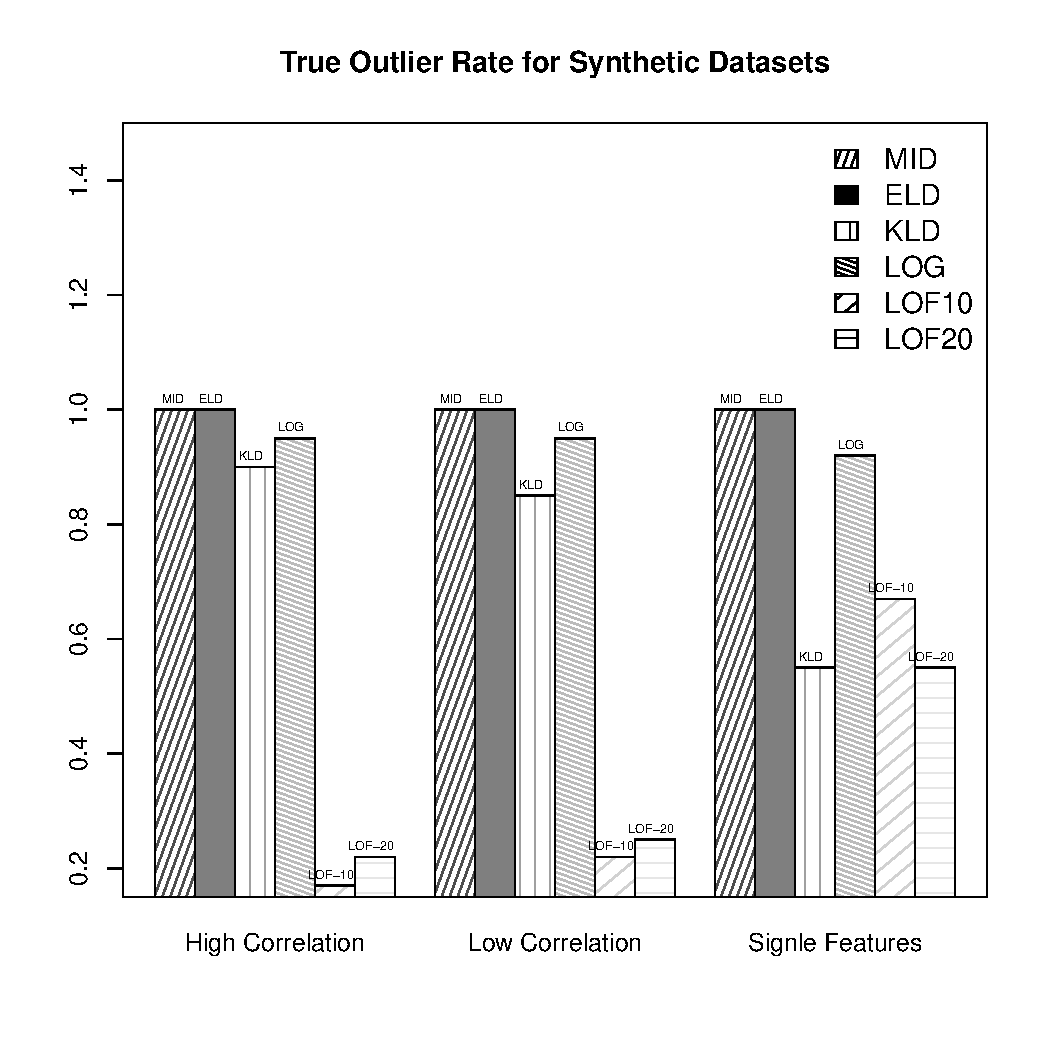
\includegraphics[height=70mm, width=70mm] {figures/TPR-Synthetic.pdf}
								%}
								%\subfigure{
								%  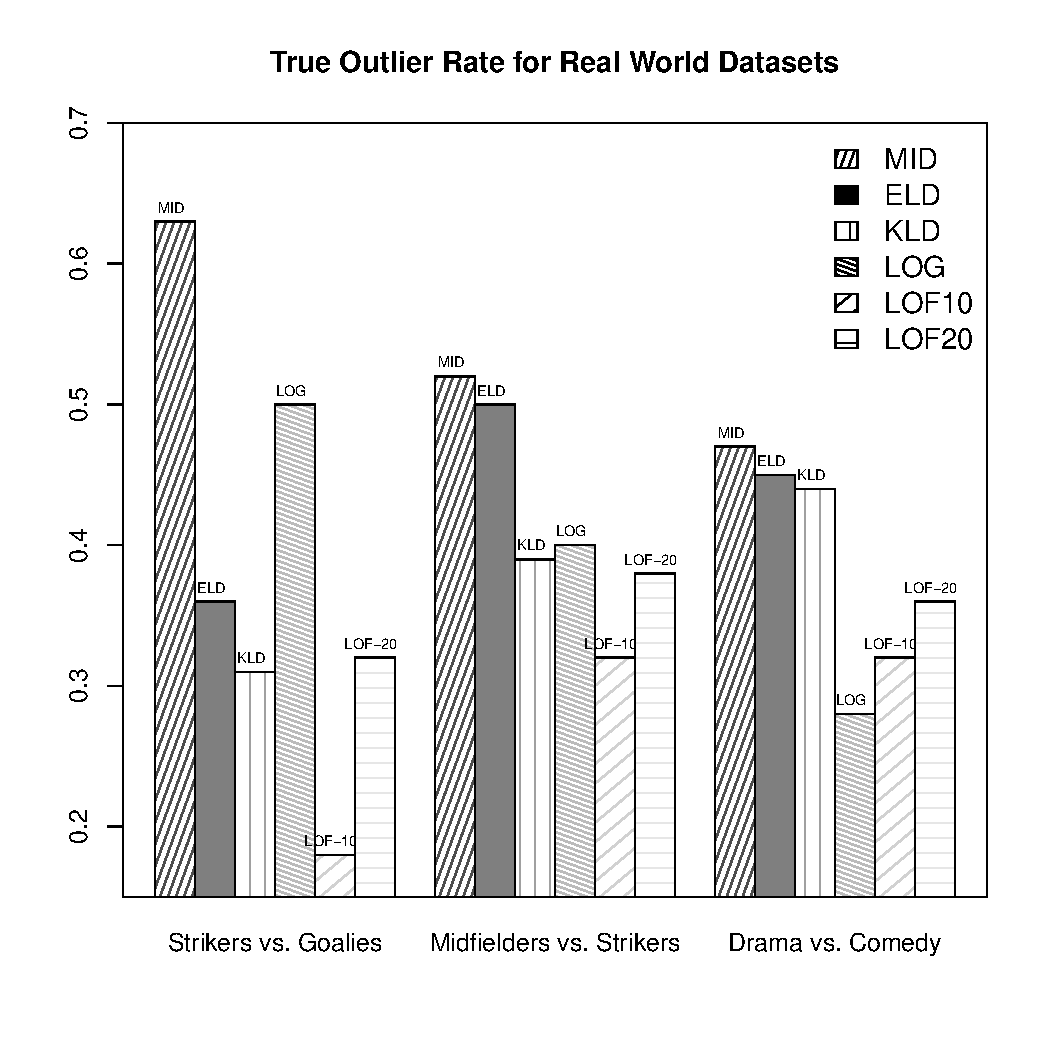
\includegraphics[height=70mm, width=70mm] {figures/TPR-All.pdf}
								
								% }
								% }
								
								%\caption{Comparison of Object Outlier Metrics}
								%\label{fig:synthetic}
								%\end{figure*}
								
								\subsubsection{Case Studies} For a case study, we examine three top outliers as ranked by $\mid$, shown in Table~\ref{table:CaseStudy}. 
								The aim of the case study is to provide a qualitative sense of the outliers discovered by the divergence scores. Also, we illustrate how the BN representation leads to an interpretable ranking. 
%								Specifically, we employ a successive decomposition of the score as follows: 
%								%{\em drill down} analysis: 
%								(1) Find the node $\feature_{i}$ that has the highest $\mid_{i}$ divergence score for the outlier object. (2) Find the parent-child combination that contributes the most to the $\mid_{i}$ score for that node. (3) Decompose the $\mid$ score for the parent-child combination into feature and mutual information component. 
								We present strong associations indicated by the mutual information component in the intuitive format of association rules.
								
								%\begin{figure}
								%\centering
								%   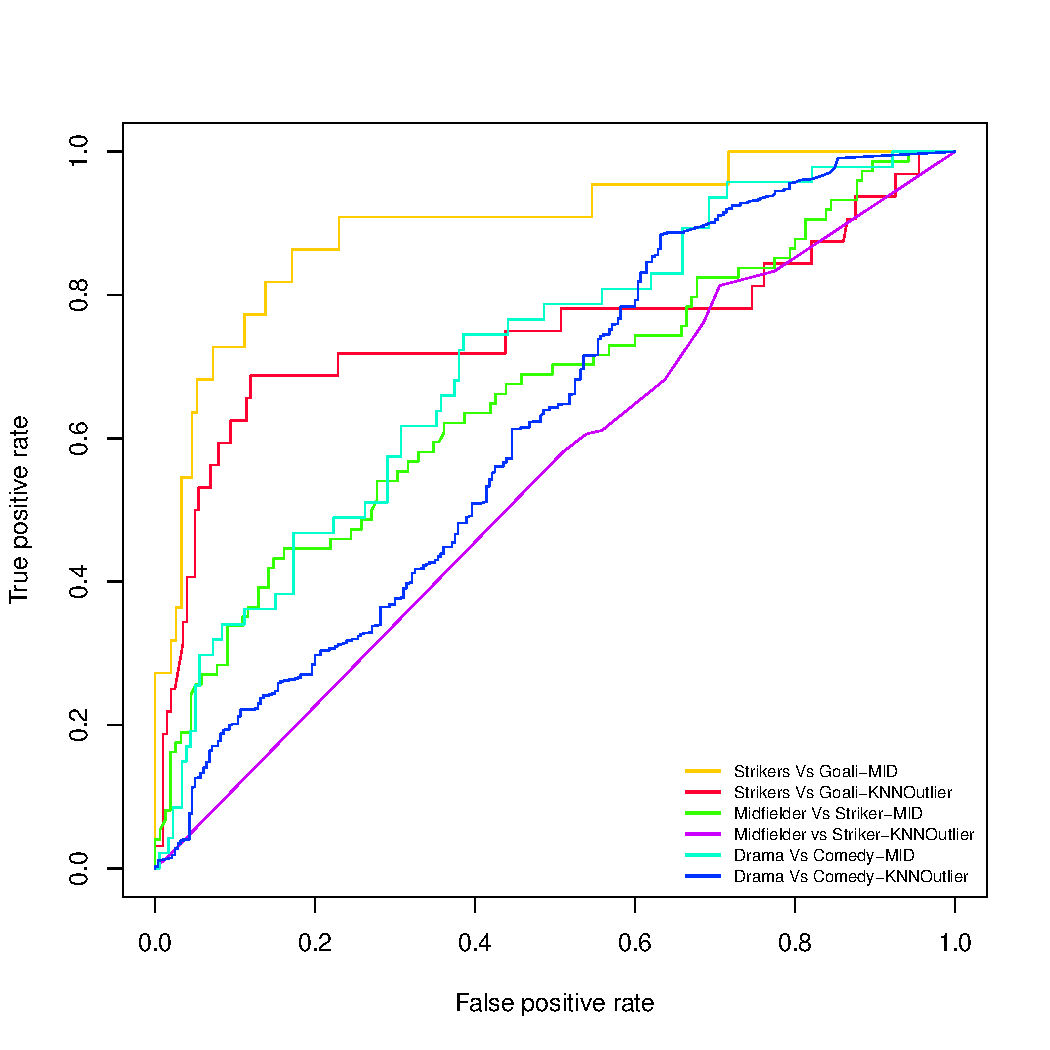
\includegraphics[width=0.5\textwidth] {figures/ROCKNN.pdf}
								% \caption{Detection Accuracy of $\mid$ vs. $\knn$
								% \label{fig:ROC}}
								%\end{figure}
								%\vspace{-5mm}
								\paragraph{Strikers vs. Goalies} 
								%The Mutual Information Divergence $\mid$ separates goalies from Strikers better compared to the other methods.  
								%
								In real-world data, a rare object may be a {\em within-class outlier}, i.e., highly anomalous even within its class. In an unsupervised setting without class labels, we do not expect an outlier score to distinguish such an in-class outlier from outliers outside the class. 
%								This is the reason why in real-world data, we do not expect an outlier detection score to distinguish the normal class objects perfectly from objects outside the class. 
								An example is the striker Edin Dzeko. He is a highly anomalous striker who obtains 
								the top $\mid$ divergence score among both strikers and goalies. His $\mid$ score is highest for the Dribble Efficiency feature. The highest $\mid$ score for that feature occurs when Dribble Efficiency is low, and its parents have the following values: Shot Efficiency high, Tackle Efficiency medium. Looking at the single feature divergence, 
								%Decomposing this $\mid$ score into feature divergence and joint information divergence, 
								we see that Edin Dzeko is indeed an outlier in the Dribble Efficiency subspace: His dribble efficiency is low in 16\% of his matches, whereas a randomly selected striker has low dribble efficiency in 50\% of their matches. Thus Edin Dzeko is an unusually good dribbler. Looking at the mutual information component of $\mid$, i.e., the parent-child correlations, for Edin Dzeko the confidence of the rule 
								$$\it{ShotEff} = \it{high}, \it{TackleEff} = \it{medium}\rightarrow \it{DribbleEff} = \it{low}$$ is 50\%, whereas in the general striker class it is $38\%$.
								%The $\eld$ divergence also ranks Edin Dzeko as unusual. But because it allows feature and joint information divergence to cancel, his rank is somewhat lower. The likelihood metric does not recognize him as unusual at all. 
								
%								The next two outliers according to $\mid$ are goalies Paul Robinson and Michel Vorm. Their rank is based only on feature divergence, with zero mutual information distinction. The maximum feature divergence is obtained by the $\it{SavesMade}$ feature. This makes intuitive sense since strikers basically never make saves. 
								%In other words, feature divergence with respect to $\it{SavesMade}$ is a good way to distinguish goalies from strikers. 
								%
								%The $\eld$ divergence also ranks Paul Robinson and Michel Vorm as clear goalies.  The likelihood metric does not recognize Paul Robinson as unusual at all. 
								%\vspace{-5mm}
								\paragraph{Midfielders vs. Strikers} 
								%The  $\mid$ metric separates midfielders from strikers better compared than the other methods.  
								%The single feature divergence does not discriminate these two classes of objects. Intuitively, this is because strikers and midfielders are generally similar with respect to single features.  
								%The distance metrics have a better TOR rate than the averaging metrics. 
								
							%	The decomposition analysis for the top three $\mid$ outliers proceeds as follows. 
								For the single feature divergence, Robin van Persie is recognized as a clear striker because of the $\it{ShotsOnTarget}$ feature. It makes sense that strikers shoot on target more often than midfielders. Robin van Persie  achieves a high number of shots on targets in $34\%$ of his matches, compared to $3\%$ for a random midfielder. The mutual information component shows that he also exhibits  unusual correlations. For example, 
								the confidence of the rule
								$$\it{ShotEff} = \it{high}, \it{TimePlayed} = \it{high} \rightarrow \it{ShotsOnTarget} = \it{high}$$
								is 70\% for van Persie, whereas in the striker class overall it is 52\%.
								%Both the $\eld$ metric and the $\lnlikelihood$ metric recognize Van Persie as a striker. 
								
%								Wayne Rooney is recognized as a striker for similar reasons, but less clearly because he achieves a high number of shots on target less frequently. 
The most anomalous midfielder is Scott Sinclair. His most unusual feature is $\it{DribbleEfficiency}$: For feature divergence, he achieves a high dribble efficiency $50\%$ of the time, compared to a random midfielder with $30\%$. 
								%The $\jid$ divergence shows that he also exhibits unusual correlations for DribbleEfficiency.
								%The $\eld$ divergence too ranks Scott Sinclair as an unusual midfielder, whereas the likelihood method places him in the middle of his class. 
								%\vspace{-5mm}
								\paragraph{Drama vs. Comedy} 
								%As with the other datasets, the  $\mid$ metric separates normal objects  from the contrast class better than the other methods.   
								The top outlier rank is assigned to the within-class outlier $\it{Brave Heart}$. Its most  unusual feature is  $\it{ActorQuality}$: In a random drama movie,  $42\%$ of actors have the highest quality level 4, whereas for $\it{Brave Heart}$ $93\%$ of actors achieve the highest quality level. 
								%The $\eld$ divergence also ranks $\it{Brave Heart}$ as an unusual drama, whereas the likelihood method places it in the middle of its class. 
								
								%based on user assigned ranking. 
								The  $\mid$ score identifies the comedies  $\it{Blues Brothers}$ and $\it{Austin Powers}$ as the top out-of-class outliers. 
							%	The main contributor to these rankings is the $\it{Cast\_Position}$ feature. 
								In a random drama movie,  $49\%$ of actors have casting position 3, whereas for $\it{Austin Powers}$ $78\%$ of actors have this casting position, and for $\it{Blues Brothers}$ $88\%$ of actors do. 
%								These three movies also show unusual correlations for this feature with high divergence in the mutual information component (not shown in Table~\ref{table:CaseStudy}).
								\begin{table*}
									\caption{Case study for the top outliers returned by \mid
										\label{table:CaseStudy}}
									\resizebox{1\textwidth}{!}{
										\begin{tabular}{|l|l|l|l|l|l|l|l|} \hline
											\multicolumn{8}{|c|}{Strikers (Normal) vs. Goalies (Outlier)}\\
											\hline
											PlayerName&Position&$\mid$ Rank&$\mid$ Max Node&$\mid$ Node Score&$\fd$ Max feature Value& Object Prob.& Class Prob. \\ \hline
											Edin Dzeko&Striker&1&DribbleEfficiency&83.84&DE=low&0.16&0.5 \\ \hline
											Paul Robinson&Goalie&2&SavesMade&49.4&SM=Medium&0.3&0.04\\ \hline
											Michel Vorm&Goalie&3&SavesMade&85.9&SM=Medium&0.37&0.04\\ \hline
											\multicolumn{8}{|c|}{Midfielders (Normal) vs. Strikers (Outlier)}\\
											\hline
											PlayerName&Position&$\mid$ Rank&$\mid$ Max Node&$\mid$ Node Score&$\fd$ Max feature Value& Object Prob.& Class Prob. \\ \hline
											Robin Van Persie& Striker&1&ShotsOnTarget&153.18&ST=high&0.34&0.03 \\ \hline
											Wayne Rooney& Striker&2&ShotsOnTarget&113.14&ST=high&0.26&0.03\\ \hline
											Scott Sinclair&Midfielder&6&DribbleEfficiency&71.9&DE=high&0.5&0.3\\ \hline
											\multicolumn{8}{|c|}{Drama (Normal) vs. Comedy (Outlier)}\\
											\hline
											MovieTitle&Genre&$\mid$ Rank&$\mid$ Max Node&$\mid$ Node Score& $\fd$ Max feature Value& Object Prob.& Class Prob. \\ \hline
											Brave Heart&Drama&1&ActorQuality&89995.4&a\_quality=4&0.93&0.42\\ \hline
											Austin Powers&Comedy&2&Cast\_Position&61021.28&Cast\_Num=3&0.78&0.49\\ \hline
											Blue Brothers&Comedy&3&Cast\_Position&24432.21&Cast\_num=3&0.88&0.49\\ \hline
										\end{tabular} 
									}
								\end{table*}
								
								%
								%\begin{table}
								%\centering
								%\tiny
								%\tabcolsep=0.11cm
								%  \begin{tabular}{|l|l|c|r| }
								%\hline
								%TeamName&Score.Imp.&Exp.Res.& Exp.Res.Diff\\ \hline
								%Swansea City&6.535&0.2971&0.0899\\ \hline
								%Tottenham Hotspur&33.0191&0.3947&0.0076\\ \hline
								%Bolton Wanderers&6.483&0.2632&0.1238\\ \hline
								%Manchester City&84.128&0.7895&0.4025\\ \hline
								%Everton&85.85&0.4211&0.0341	\\ \hline	
								%  \end{tabular}
								%\caption{Data for premier league teams with significant score improvement: Score Improvement, Expected result of the team (model estimate), Expected Result Difference from team population mean (0.38).}
								%\label{table:team}
								%\end{table}
								
								%\section{Outlier Metric}
								%In this section we introduce and motivate an outlier metric that we apply for identifying atypical individuals. In a nonrelational dataset with unrelated invidiuals, an individual is represented as a data point or attribute vector. In a relational data structure, an individual may differ from others not only in its attributes, but also in its links and in the attributes of linked entities. This means that the data for an individual may exhibit statistical correlations, or associations, that differ from those in the general population. We may term such individuals {\em association outliers.} For instance, we may find that among teams in general, dribble effiency does not predict the pass efficiency of  a team,  but that it does for Manchester City in particular. \marginpar{match up with rules}. The fact that an individual may show unusual associations as well as unusual attributes is a special feature of relational data. To compactly represent statistical associations valid for an individual, we learn a graphical  model for the subdatabase associated with the individual, termed the {\em individual model}.  In a Bayes net model, probabilistic associations can often be interpreted causally \cite{Pearl}. For example in the sports domain, a Bayes net can suggest what the causal drivers of a team's performance are.
								%
								%
								%Our basic approach to measuring the atypicality of an individual is to compare a graphical model learned for the entire population---termed the {\em generic model}---to an individual model. There are various options for defining a metric between two models. We propose to make use of standard model selection scores from statistics. Such scores measure how well a model fits a dataset. Our proposal is to use the difference between the score of the individual Bayes net on the individual's data, and the generic Bayes net applied to the individual's data. The intuition is that the worse the generic Bayes net fits the individual data, the more the individual differs from the general population. To define the score-difference metric formally, we introduce some notation.
								%[...]
								%
								%Advantages to the score-difference metric include the following.
								%
								%\begin{enumerate}
								%\item Based on fundamental statistical concepts.
								%\item Aggregates all the available information about links and attributes.
								%%\item Sensitive to differences in statistical and causal dependencies valid for the individual vs. those valid in the general population.
								%\item Can be decomposed into scores for specific attributes and further into scores for values of those attributes.
								%\end{enumerate}
								%
								%Decomposability is important because it provides the user with the option of investigating the components of the outlier metric to understand the result of the metric in detail, rather than just reporting a single number. To this end we introduce a {\em drill-down} methodology for analyzing an association outlier at different scales. 
								%
								%\begin{enumerate}
								%\item The score-difference for an individual Bayes net is the sum of score-differences for the nodes in the Bayes net.
								%\item The score for a child node is the sum of scores over the possible values of parents and the child. The score can be used to select associations between values of parents and the child, which can be represented in association rule form.
								%\end{enumerate}
								% 
								%[By subtracting the common trend, the individual deviations that do exist become more pronounced.] 
								%
								%1. Define log-likelihood formally, with frequencies.
								%
								%Discuss frequencies.
								%The log-likelihood metric is a basic ingredient in standard model selection scores. For instance, the AIC score is defined as ....
								%
								%
								%\paragraph{Synthetic Data} 
								%We generate Synthetic data based on Premier league data structure using $\it{mlbench}$ package in $\it{R}$. By using this package, different classes can be generated and are uniformly distributed on the d-dimensional cube with corners. We used a 2-class problem. The first class is a d-dimensional ball in the middle of the cube (non-outlier) and the remainder forms the second class (outlier). The size of the ball is chosen such that both classes have equal prior probability 0.5. Then, for each data point, we sample a continuous vector based on the label of each data point. For synthetic data type one, we assumed that each team has a fixed number of outlier players while in synthetic data type two, we generated two teams such that all their players are outliers \cite{Pei2006}. 
								
								\subsubsection{Details on Systems and Algorithms} 
\label{sec:details}
%We provide details about systems and algorithms that we use from previous work. 
All the experiments were performed on a 64-bit Centos machine with 4GB RAM and an Intel Core i5-480 M processor. The likelihood-based outlier scores were computed with SQL queries invoked by JDBC, JRE 1.7.0. and MySQL Server version 5.5.34.


\paragraph{Bayesian Network Learning}
				\label{sec:bnlearning}
				
%				To compactly represent the class and object distributions, we 
%				use object-oriented Bayesian networks \cite{Koller1997}. 
%				%Unfortunately, 
%				To our knowledge no structure learning methods for object-oriented BNs have been developed. We therefore adapt for object-oriented data 
%				a previously developed  method that learns a BN for a relational database. 
				%This approach exploits the  fact that object-oriented data can be translated into relational data tables \cite[Ch.27.8.1]{Ramakrishnan2003}. 
				%An analogous approach is taken by some object-oriented database systems for query processing: Given a query for object data translated the data into a set of relational tables, and the query into a standard SQL query \cite[Ch.27.8.1]{Ramakrishnan2003}. 
				%
				We utilize the learn-and-join algorithm (LAJ), which is
				a state-of-the-art BN structure learning method for relational data \cite{Schulte2012}. The LAJ algorithm employs an iterative deepening strategy, which can be described as follows for object data. The algorithm learns a set of interrelated BNs. The initial step is to learn one BN for each object class. The BN for one class represents associations among the features of the objects in the class only. Then the algorithms learns a BN for each pair of linked components, such that the BN for the pair inherits the edges of the BNs for the objects. Next the algorithm learns a BN for each triple of  objects related by a path of length 2, where edges are inherited from the BNs for the relevant pairs, etc. The algorithm stops when increasing the path length leads to no new edges being learned. The multiple Bayesian networks are then merged into a complete Bayesian networks for all objects. For a full description, complexity analysis, and learning time measurements, please see \cite{Schulte2012}. 
				%
				%To illustrate, a possible run of the LAJ algorithm in the example data of Section~\label{sec:object-distributions} would be.
				%
				The Bayesian network parameters for a target object distribution can be learned in the same way, where the input data is the object profile rather than the entire dataset. 
				We used the implementation of the LAJ algorithm due to its creators \cite{bib:jbnsite}. 

\paragraph{Single-Matrix Based Outlier Detection Methods} 
%We describe the details of the standard i.i.d. outlier detection methods we used.
The $\outrank$ research of~\cite{Muller2012} suggests that \textit{PRO-CLUS} is the best clustering function for their approach. Our experiments applied $\outrank$ with two subspace clustering models, \textit{PRO-CLUS} \cite{Muller2012} and \textit{DISH} \cite{Kriegel2007}.  
						We used the available implementation of all three data matrix methods from the state of the art data mining software \textit{ELKI} \cite{Elke2013}.
								

\section{Related Work}

%[subgroup detection exceptional model mining vs. outlier = subgroup of size 1]

%[global outlier]
%Whenever a data point notably deviates from the rest of population, it is categorized as global outlier. This type of outliers are the simplest and finding them is the target of most of outlier detection methods. The main challenge of this type of outlier is that sometimes it is hard to find an appropriate measurement of deviation.


Outlier detection is a densely researched field, for a survey please see~\cite{aggarwal2013}.
Figure~\ref{fig:novelty} provides a graphical picture of where our method is situated with respect to other outlier detection methods and other data models. 
%For an outlier detection survey please see~\cite{aggarwal2013}.
%\cite{Hodge2004,aggarwal2013}. 
Our method falls in the category of {\em unsupervised} statistical model-based approaches. To our knowledge, ours is the first model-based method tailored for object-relational data. Like other model-based approaches, it detects global outliers. \cite{aggarwal2013} defines a global outlier to be a data point that notably deviates from the rest of population. We review relevant approaches from different data models, the most common atomic object model---where data is represented by a single data matrix---and structured data models using the XML, SQL, and OLAP formats.
%\vspace{-5mm}
\paragraph{Atomic Objects; Attribute Vector Data Model}

By far most work on outlier detection considers atomic objects with flat feature vectors.
%, or nonhierarchical structures like time series. 
This leads to an impedance mismatch: The required input format for these outlier detection methods is a single data matrix, not a structured dataset. For example, one cannot provide a relational database as input. This is not simply a question of choosing a file format, but instead reflects a different underlying data model.
%: complex objects with both attributes and component objects vs. atomic objects with attributes only. 
%
It is possible to ``flatten'' structured data by converting it to unstructured feature vectors, for instance by using aggregate functions. Flattening incurs some loss of information but allows us to apply the many feature vector methods.
%\cite{Elke2013}. 
We evaluate the aggregation approach in this paper by using standard methods for three major approaches to outlier detection: distance-based, density-based, and subspace clustering. 

%Subspace clustering methods (e.g., \cite{Muller2012,Kriegel2009}) are similar to our work in the sense that they aim to decompose a complex data space. They find complex deviations that are noticeable only in a data subspace. A common approach is to discover datapoints that show unexpected deviations in similar subspaces. Our approach instead develops a joint measure of how dissimilar the target object profile distribution is to the class distribution over the entire data space. Given that object and class distributions are represented by an object-oriented Bayesian network \cite{Koller1997}, the network structure defines subspaces. The joint divergence measure {\em mathematically decomposes} into subspace measures that quantify how dissimilar the target object profile distribution is in the subspaces defined by the network, compared to the class distribution in the same subspace.

Work on atomic contextual  outliers \cite{Tang2013} is like ours in that it considers the distinctness of a target individual from a reference class. A reference class is not specified as a property of the object, but is constructed as part of outlier detection. 
%Our work could be combined with a class discovery approach by providing a score of how informative the inferred classes are. 
\begin{figure}
	\centering
	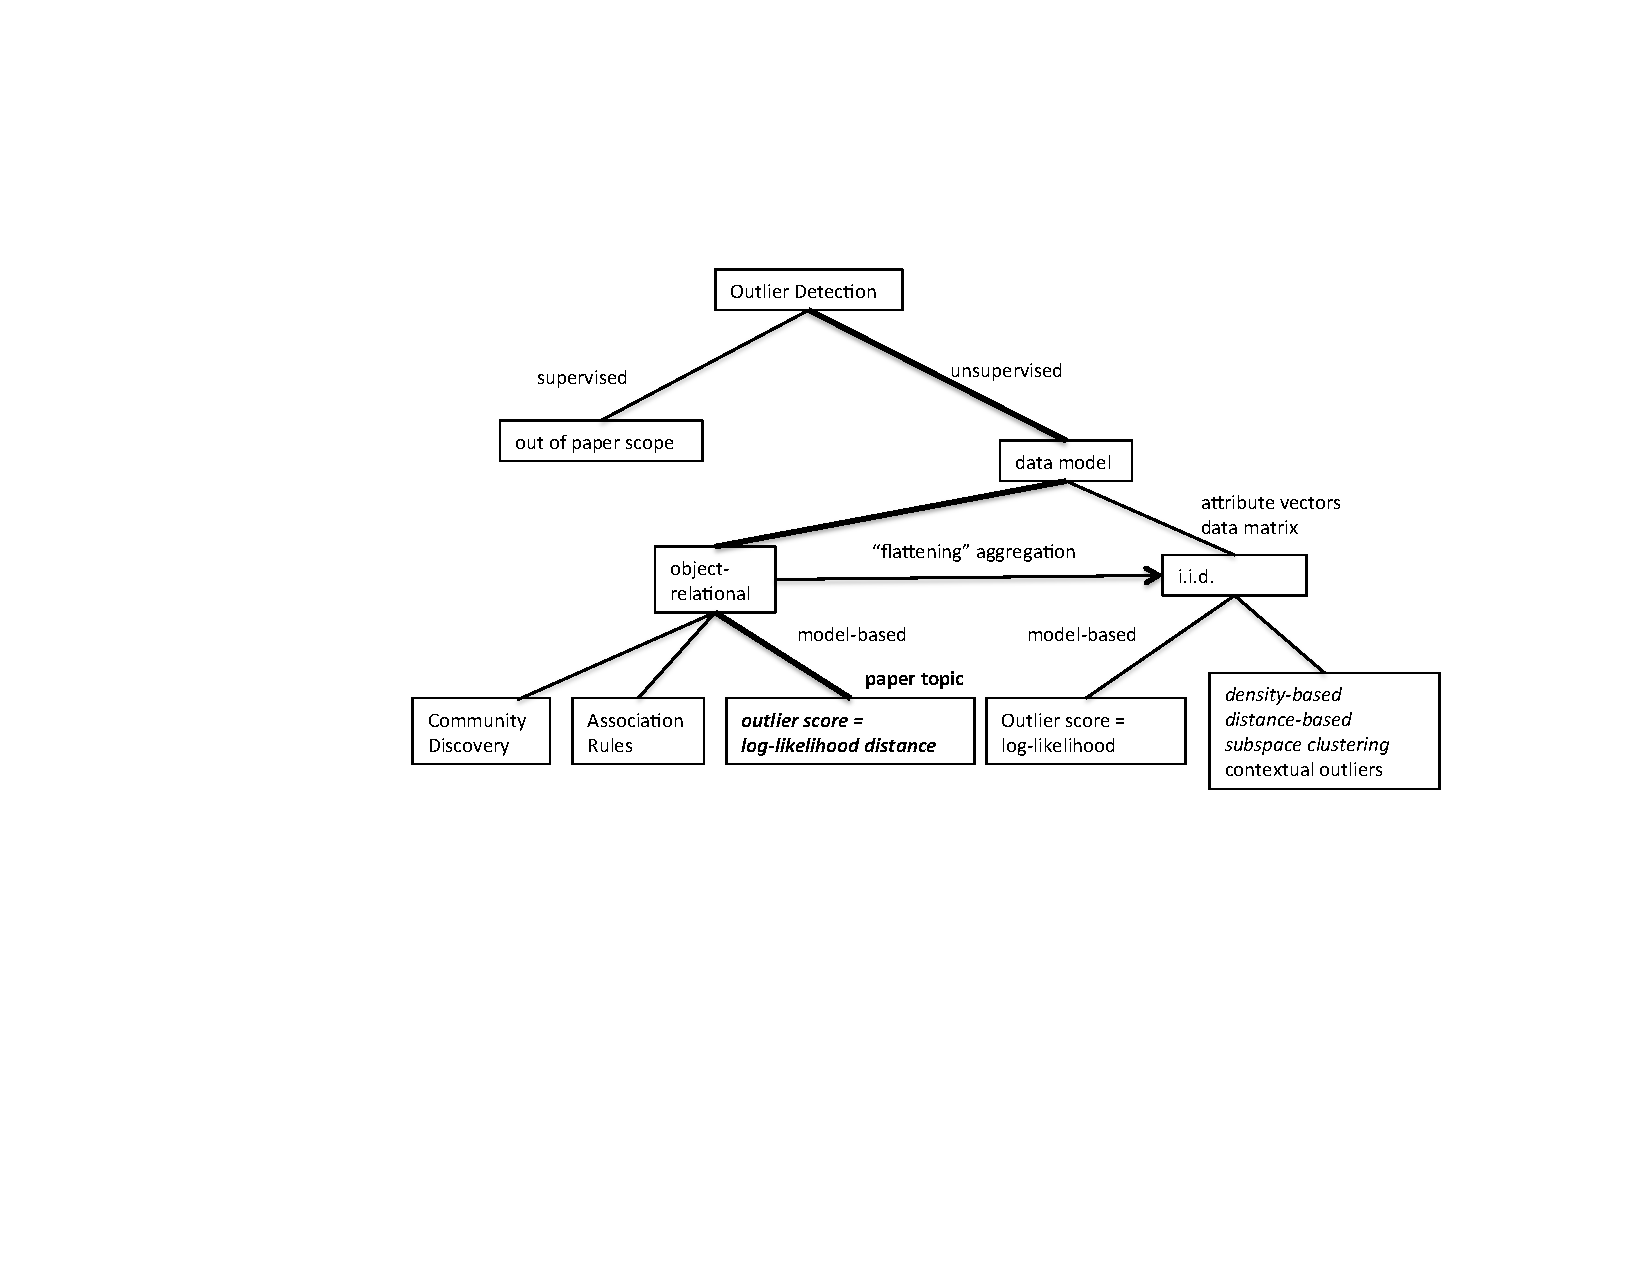
\includegraphics[width=0.5\textwidth] {NoveltyDiagram}
	\caption{A tree structure for related work on outlier detection for structured data. A path specifies an outlier detection problem, the leaves list major approaches to the problem. Approaches in italics appear in experiments.
		\label{fig:novelty}}
\end{figure}
%\vspace{-5mm}
\paragraph{Structured Data Models} We discuss related techniques in three types of structured data models: SQL (relational data), XML, and OLAP (multi-dimensional data). 

For relational data, many outlier detection approaches aim to discover rules that represent the presence of anomalous associations for an individual or the absence of normal associations \cite{Maervoet2012,Gao2010}. Such local rules are informative, but they are not based on a global statistical model and do not provide a single outlier score for each individual. The survey by \cite{Novak2009} unifies within a general rule search framework related tasks such as exception mining, which looks for associations that characterize unusual cases, subgroup mining, which looks for associations  characterizing important subgroups, and contrast space mining, which looks for differences between classes.  A latent variable approach in information networks ranks potential outliers in reference to the latent communities inferred by network analysis \cite{Gao2010}. Our model aggregates information from entities and links of different types, but does not assume that different communities have been identified. 


Koh {\em et al.}~\cite{Koh2008} propose a method for hierarchical structures represented in XML document trees. Their aim is to identify feature outliers, not class outliers as in our work. Also, they use aggregate functions to convert the object hierarchy into feature vectors. Their outlier score is based on local correlations, they do not construct a model.


The multi-dimensional data model defines numeric measures for a set of dimensions. A seminal approach to exploring a multi-dimensional datacube was presented by Sarawagi {\em et al.}~\cite{Sarawagi1998}. 
%The object and the multi-dimensional data models are similar in the respect that both objects and dimensions are ordered in a hierarchy. However, 
The differences in the two data models mean that multi-dimensional outlier detection models do not carry over to object-relational outlier detection. (1) The object data model allows but does not require any numeric measures. In the datasets we examine in this paper, all features are discrete. Nor do we assume that it is possible to aggregate numeric measures to summarize lower-level data at higher levels.  
%(2) In scoring a potential outlier object, our method considers other objects {\em both} below and above the target object in the component hierarchy. OLAP exploration methods consider only cells below or at the same level as the target cell. For example, in scoring a player, our method would consider features of the player's team.  
%(3) The outlier score of an object is not determined by the outlier scores of its components. By contrast, the approach of Sarawagi {\em et al.} considers values such as the most unusual cell that is below a target cell. 
(2) Our approach models a joint distribution over features, exploiting correlations among features. Most of the OLAP-based methods consider only a single numeric measure at a time, not a joint model. 
								
								
\section{Conclusion} We presented a new approach for applying Bayes nets to object-relational outlier detection. The key idea is to learn one set of parameter values that represent class-level associations, another set to represent object-level associations, and compare how well each parametrization fits the relational data that characterize the individual. The classic metric for comparing two parametrized models is their log-likelihood ratio; we refined this concept to define  a new relational log-likelihood distance metric via two transformations:  (1) a mutual information decomposition, and (2) replacing log-likelihood differences by log-likelihood distances. This metric combines a single feature component, where features are treated as independent, with a correlation component that measures the deviation in the features' mutual information.

In experiments on three synthetic and three real-world outlier sets, the log-likelihood distance achieved the best true positive and true negative rates. The alternative of converting the structured data to a flat data matrix via aggregation had a negative impact on outlier detection. Case studies showed that the log-distance score leads to easily interpreted rankings.
%
Overall, our new log-likelihood distance metric provides a promising new approach for applying machine learning techniques to outlier detection for object-relational data, a challenging and practically important topic. 

 							
								There are several avenues for future work.  A limitation of our current approach is that it ranks potential outliers, but does not set a threshold for a binary identification of outlier vs. non-outlier. Our divergence uses expected L1-distance for interpretability, but other distance scores like L2 could be investigated as well. Extending the expected L1-distance for continuous features is a useful addition. 
								%, and may facilitate combining our object-oriented approach with dimensional hierarchies in an OLAP data cube.
								%Distribution distances other than KLD could be evaluated for outlier detection (e.g., variation distance). However, the KLD variants have special advantages: their asymetry reflects the asymetry between object and class. Also, in a Bayesian network representation of the joint distributions, they decompose into a node-wise sum for easy computation and interpretation. 
								%A promising project for future work would be to combine the object data model and the multi-dimensional model to combine our object outlier method with OLAP-based methods. For example, one could add numeric measures and aggregate attributes to the object model. Another view: convert the object-oriented data to OLAP data, then use their outlier detection.
								
								
								In sum, outlier metrics based on model likelihoods are a new type of structured outlier score for object-relational data. Our evaluation indicates that this type of score provides informative, interpretable, and accurate rankings of objects as potential outliers.
								
								
								\bibliographystyle{abbrv}
								\bibliography{Bibliography-File,master}
							\end{document}
							
							
							


% conference papers do not normally have an appendix


% use section* for acknowledgement
\section*{Acknowledgment}


The authors would like to thank NSERC.\footnote{copy from UAI paper}

 

% trigger a \newpage just before the given reference
% number - used to balance the columns on the last page
% adjust value as needed - may need to be readjusted if
% the document is modified later
%\IEEEtriggeratref{8}
% The "triggered" command can be changed if desired:
%\IEEEtriggercmd{\enlargethispage{-5in}}

% references section

% can use a bibliography generated by BibTeX as a .bbl file
% BibTeX documentation can be easily obtained at:
% http://www.ctan.org/tex-archive/biblio/bibtex/contrib/doc/
% The IEEEtran BibTeX style support page is at:
% http://www.michaelshell.org/tex/ieeetran/bibtex/
%\bibliographystyle{IEEEtran}
% argument is your BibTeX string definitions and bibliography database(s)
%\bibliography{IEEEabrv,../bib/paper}
%
% <OR> manually copy in the resultant .bbl file
% set second argument of \begin to the number of references
% (used to reserve space for the reference number labels box)
\begin{thebibliography}{1}

\bibitem{IEEEhowto:kopka}
H.~Kopka and P.~W. Daly, \emph{A Guide to \LaTeX}, 3rd~ed.\hskip 1em plus
  0.5em minus 0.4em\relax Harlow, England: Addison-Wesley, 1999.

\end{thebibliography}




% that's all folks
\end{document}


